\documentclass[11pt,a4paper]{article}

\usepackage[T1]{fontenc}
\usepackage[utf8]{inputenc}
\usepackage[spanish,es-noshorthands,es-nodecimaldot,es-tabla]{babel}
\usepackage{lmodern}
\usepackage{microtype}
\usepackage[margin=2.5cm]{geometry}
\usepackage{amsmath,amssymb,amsthm,mathtools}
\usepackage{booktabs}
\usepackage{graphicx}
\usepackage{xcolor}
\usepackage{listings}
\usepackage{tikz}
\usetikzlibrary{positioning}
\usepackage{enumitem}
\usepackage[hidelinks]{hyperref}

\definecolor{codebg}{RGB}{247,247,249}
\definecolor{codekw}{RGB}{0,92,170}
\definecolor{codecm}{RGB}{110,110,110}
\lstset{
  language=Python, basicstyle=\ttfamily\small, backgroundcolor=\color{codebg},
  keywordstyle=\color{codekw}\bfseries, commentstyle=\color{codecm}\itshape,
  stringstyle=\color{teal!70!black}, frame=single, rulecolor=\color{black!15},
  breaklines=true, columns=fullflexible, keepspaces=true, showstringspaces=false,
  xleftmargin=4pt, xrightmargin=4pt, aboveskip=8pt, belowskip=8pt
}

\theoremstyle{plain}
\newtheorem{proposicion}{Proposición}[section]
\newtheorem{corolario}[proposicion]{Corolario}
\theoremstyle{remark}
\newtheorem*{observacion}{Observación}

\newcommand{\fn}[1]{\texttt{\detokenize{#1}}}
\newcommand{\Z}{\mathbb{Z}}
\newcommand{\R}{\mathbb{R}}
\newcommand{\Lgen}{\mathcal{L}}
\DeclareMathOperator{\sgn}{sgn}
\DeclareMathOperator{\diag}{diag}
\newcommand{\norm}[1]{\lVert #1\rVert}
\newcommand{\ip}[2]{\langle #1,#2\rangle}

\title{Explicación del notebook\\[4pt]
\large Simulación del proceso de ramificación en complejos celulares}
\author{Martín Maturana Acevedo\\[2pt]\small Proyecto de Simulación Estocástica --- basado en el borrador de D.~Cid y A.~Sepúlveda}
\date{Octubre 2026}

\begin{document}
\maketitle

\begin{abstract}
Este documento explica, sección por sección, el notebook \fn{branching_process_complexes.ipynb}, que simula el proceso de ramificación sobre el complejo cúbico $\Z^d$ descrito en el borrador \emph{Branching process on complexes}. Para cada parte se explica qué objeto matemático se construye, cómo se implementa y por qué de esa forma. El documento también reúne las \textbf{verificaciones numéricas de la teoría} ($\partial\partial=0$, Laplacianos, drift, desigualdad de Lyapunov, Poincaré), que ya no están en el notebook; su código está en el Apéndice~\ref{app:codigo}. El resultado central es un \textbf{teorema de cargas conservadas}: para cada componente conexa del grafo de aristas absorbentes, el flujo neto de partículas que sale de ella se conserva, y la extinción es posible si y solo si todos esos flujos son nulos. Con él se estudia cómo varía la probabilidad de extinción al agregar aristas absorbentes. Ese estudio muestra que la extinción eventual es monótona en el conjunto absorbente, pero la extinción en tiempo finito no lo es. Finalmente, la \S\ref{sec:fundamentos} explica con detalle los fundamentos de la simulación y de la estimación (exactitud del algoritmo de Gillespie, estimador de Bernoulli, censura, intervalos de Wilson, cálculo exacto vía cargas y teoría cuasi-estacionaria) y reúne preguntas frecuentes para la presentación.
\end{abstract}

\tableofcontents
\newpage

%=====================================================================
\section{Visión general}
%=====================================================================

\subsection{El modelo}

Sobre las aristas de una grilla cúbica hay partículas con carga. Una configuración es un vector de enteros
\[
\theta\in\Theta=\Z^{E^+},
\]
con una entrada por arista (positivamente orientada): $\theta(e)=3$ significa tres partículas positivas en $e$, y $\theta(e)=-2$ significa dos partículas negativas. En cada evento:
\begin{enumerate}[nosep]
  \item se elige una partícula, digamos en la arista $e$;
  \item se elige una cara $f$ (un cuadradito) que tenga a $e$ en su borde;
  \item la cara \emph{suena}: a $\theta$ se le resta su borde orientado, con un signo $c=\pm1$ escogido para que la partícula de $e$ se cancele,
  \[
  \theta\;\longmapsto\;\theta-c\,\partial f,\qquad c=\ip{e}{\partial f}\sgn(\theta_e).
  \]
\end{enumerate}
Como el borde de un cuadrado tiene $\beta=4$ aristas, la partícula original desaparece y nacen $\beta-1=3$ partículas en los otros lados: esa es la \emph{ramificación}. Si una carga nueva llega a una arista con carga opuesta, ambas se cancelan: esa es la \emph{aniquilación}. El generador del proceso es
\[
\Lgen\phi(\theta)=\sum_{e\in E^+}|\theta_e|\sum_{f\ni e}\Big(\phi\big(\theta-\ip{e}{\partial f}\sgn(\theta_e)\,\partial f\big)-\phi(\theta)\Big).
\]

\subsection{Flujo del notebook}

\begin{center}
\begin{tikzpicture}[node distance=4mm, every node/.style={draw, rounded corners, fill=black!4, font=\small, align=center, minimum height=8mm}]
\node (a) {grilla\\(celdas)};
\node[right=of a] (b) {$\partial_1,\partial_2$\\matrices};
\node[right=of b] (c) {Laplacianos};
\node[right=of c] (d) {conjunto\\absorbente $T$};
\node[below=8mm of d] (e) {simulación\\(solo eventos)};
\node[left=of e] (f) {reconstrucción\\de $\theta_t$};
\node[left=of f] (g) {verificación\\de teoremas};
\node[left=of g] (h) {videos};
\foreach \x/\y in {a/b,b/c,c/d,d/e,e/f,f/g,g/h} \draw[->, thick] (\x) -- (\y);
\end{tikzpicture}
\end{center}

\subsection{Organización actual del notebook}

El notebook contiene la implementación, los videos y el estudio de extinción. Las verificaciones básicas viven en este documento. Sus secciones son:
\begin{enumerate}[nosep]
  \item complejo cúbico y operadores (\S\S2--4 de este documento);
  \item absorción (\S5);
  \item motor estocástico (\S6);
  \item configuraciones iniciales y reconstrucción (\S\S6--7);
  \item visualización 2D y 3D (\S8);
  \item réplicas, condiciones iniciales y absorción (\S9);
  \item videos (\S10);
  \item probabilidad de extinción según el número de aristas absorbentes (\S11).
\end{enumerate}

\subsection{Principios de diseño}

\begin{itemize}[nosep]
  \item \textbf{Responsabilidad única}: muchas funciones pequeñas, cada una con un solo trabajo y un nombre que lo describe.
  \item \textbf{Álgebra lineal rala}: todos los operadores (frontera, co-frontera, Laplacianos) son matrices de \fn{scipy.sparse}. Casi todas sus entradas son cero; cada columna de $\partial_2$ tiene solo 4 entradas no nulas.
  \item \textbf{Vectorización}: el único bucle de la simulación es el del tiempo, que es inevitable porque una cadena de Markov es secuencial. Dentro de cada paso todo es vectorizado o de costo constante.
  \item \textbf{Reproducibilidad}: toda la aleatoriedad pasa por \fn{np.random.default_rng(seed)}, y en los experimentos de extinción cada réplica tiene su propia semilla, de modo que el cómputo en paralelo da exactamente lo mismo que en serie.
\end{itemize}

\paragraph{La celda de imports.} Lo único no estándar es \fn{scipy.sparse} (matrices ralas), \fn{scipy.sparse.csgraph} (algoritmos de grafos sobre matrices ralas, usados para el árbol generador) y \fn{matplotlib.animation} (videos). La variable \fn{VIDEO_DIR} crea la carpeta \fn{videos/}.

%=====================================================================
\section{Topología: cómo se representan las celdas}
%=====================================================================

\subsection{Coordenadas semienteras y coordenadas dobladas}

Siguiendo la ecuación~(1) del paper, cada $k$-celda positiva de $\Z^d$ se identifica con su baricentro:
\[
\Xi_k^+\Z^d=\Big\{x+\tfrac12\chi_J\;:\;x\in\Z^d,\ J\in\tbinom{[d]}{k}\Big\}\subset\tfrac12\Z^d,\qquad \chi_J=\sum_{j\in J}e_j .
\]

\begin{center}
\begin{tabular}{@{}llll@{}}
\toprule
celda & ejemplo & baricentro & doblado \\
\midrule
vértice & el punto $(2,2)$ & $(2,2)$ & $(4,4)$ \\
arista & de $(1,2)$ a $(2,2)$ & $(\tfrac32,2)$ & $(3,4)$ \\
cara & $[1,2]\times[0,1]$ & $(\tfrac32,\tfrac12)$ & $(3,1)$ \\
\bottomrule
\end{tabular}
\end{center}

La observación clave es que \textbf{la dimensión de una celda es la cantidad de coordenadas estrictamente semienteras de su baricentro}: un vértice no tiene ninguna, una arista tiene una (y esa coordenada indica su dirección), una cara tiene dos.

Para no trabajar con decimales, el código usa \emph{coordenadas dobladas} $z=2x\in\Z^d$. Así, ``semientera'' se convierte en ``impar'', y una caja $[0,n_1]\times\cdots\times[0,n_d]$ corresponde a la grilla de enteros
\[
\{0,\dots,2n_1\}\times\cdots\times\{0,\dots,2n_d\},
\]
en la que \textbf{cada punto es exactamente una celda}, de dimensión igual a su número de coordenadas impares.

\subsection{Las funciones}

\begin{description}[style=nextline, leftmargin=1.2em, font=\normalfont]
  \item[\fn{doubled_grid_shape(box_shape)}] Tamaño de la grilla doblada: $(2n_1+1,\dots,2n_d+1)$. Para la caja $(3,3)$ devuelve $(7,7)$.
  \item[\fn{all_doubled_points(box_shape)}] Todos los puntos de la grilla doblada como arreglo de $N\times d$, usando \fn{np.indices}.
  \item[\fn{cell_dimensions(points)}] Cuenta las coordenadas impares de cada punto: \texttt{points \% 2} vale 1 en las impares y \fn{count_nonzero} las suma por fila.
  \item[\fn{cells_of_dimension(box_shape, k)}] Filtra los puntos de dimensión $k$.
  \item[\fn{build_vertices}, \fn{build_edges}, \fn{build_faces}] Llaman a la anterior con $k=0,1,2$. Son de una línea; existen para que cada responsabilidad tenga nombre propio.
  \item[\fn{build_cell_lookup(cells, box_shape)}] Tabla inversa: dada una coordenada, entrega la posición de esa celda en su lista. Es un arreglo plano del tamaño de toda la grilla, inicializado en $-1$; \fn{np.ravel_multi_index} convierte una coordenada $(i,j)$ en un índice lineal (como al aplanar una matriz) y en esas posiciones se escribe $0,1,2,\dots$
  \item[\fn{lookup_cells(coords, lookup, box_shape)}] Usa la tabla para buscar muchas celdas a la vez, sin bucles.
\end{description}

Una consecuencia importante es que \textbf{las celdas siempre quedan en el mismo orden} (lexicográfico). Así ``la arista número 37'' significa siempre lo mismo, y el vector $\theta$ queda bien definido.

%=====================================================================
\section{Operadores de frontera y co-frontera}
%=====================================================================

\subsection{La fórmula del borde}

La Definición~1.5 del paper da el borde de una $k$-celda $x$:
\[
\partial_k x=\sum_{i\in J_x}\varepsilon_{J_x}(i)\,\big(x^{+i}-x^{-i}\big),\qquad
x^{\pm i}=x\pm\tfrac12e_i,\qquad
\varepsilon_J(s)=(-1)^{\#\{j\in J\,:\,j<s\}},
\]
donde $J_x$ es el conjunto de direcciones semienteras de $x$. Moverse $\pm\frac12 e_i$ en una dirección semientera la vuelve entera, así que se baja una dimensión: se llega a una cara del borde. En coordenadas dobladas, $x^{\pm i}$ es simplemente $z\pm e_i$.

El signo $\varepsilon_J(i)$ es el signo de la transposición que lleva $dx_i$ al frente de $dx_{j_1}\wedge\cdots\wedge dx_{j_k}$: se cuentan cuántas direcciones de $J$ están \emph{antes} de $i$.

\subsection{Ejemplo: el cuadrado unitario}

Para la cara $x=(\frac12,\frac12)$, doblada $(1,1)$, se tiene $J=\{1,2\}$.

\noindent\textit{Dirección horizontal.} Para $i=1$ no hay elementos de $J$ antes de $1$, así que $\varepsilon=+1$: aparece $+(1,\frac12)$, la arista derecha, y $-(0,\frac12)$, la arista izquierda.

\noindent\textit{Dirección vertical.} Para $i=2$ la dirección $1$ está antes, así que $\varepsilon=-1$: aparece $-(\frac12,1)$, la arista de arriba, y $+(\frac12,0)$, la arista de abajo.

\begin{center}
\begin{tikzpicture}[scale=2.2, >=stealth]
\fill[black!6] (0,0) rectangle (1,1);
\draw[->, very thick, red!70!black] (0,0) -- (1,0) node[midway, below] {$+x^{-2}$ (abajo)};
\draw[->, very thick, red!70!black] (1,0) -- (1,1) node[midway, right] {$+x^{+1}$ (derecha)};
\draw[->, very thick, blue!70!black] (0,1) -- (1,1) node[midway, above] {$-x^{+2}$ (arriba)};
\draw[->, very thick, blue!70!black] (0,0) -- (0,1) node[midway, left] {$-x^{-1}$ (izquierda)};
\node at (0.5,0.5) {$x$};
\draw[->, thin, black!50] (0.5,0.5) ++(0.22,0) arc (0:300:0.22);
\end{tikzpicture}
\end{center}

Las flechas indican la orientación canónica de cada arista (hacia la derecha y hacia arriba). Abajo y derecha entran con $+$; arriba e izquierda entran con $-$, es decir, se recorren al revés. El resultado es el \textbf{borde recorrido en sentido antihorario}:
\[
\partial_2 x = x^{-2}+x^{+1}-x^{+2}-x^{-1}.
\]
El signo $\varepsilon$ existe precisamente para que las orientaciones encajen así, y es lo que hace que $\partial\partial=0$.

\subsection{Implementación}

\begin{lstlisting}
def orientation_sign(cells, i):
    below = np.count_nonzero(cells[:, :i] % 2, axis=1)
    return 1 - 2 * (below % 2)

def boundary_entries_in_direction(cells_k, lookup_km1, box_shape, i):
    cols = np.flatnonzero(cells_k[:, i] % 2 == 1)   # celdas con i en J_x
    x = cells_k[cols]
    shift = np.zeros(cells_k.shape[1], dtype=np.int64)
    shift[i] = 1
    eps = orientation_sign(x, i)
    plus = lookup_cells(x + shift, lookup_km1, box_shape)
    minus = lookup_cells(x - shift, lookup_km1, box_shape)
    return (np.concatenate([plus, minus]), np.concatenate([cols, cols]),
            np.concatenate([eps, -eps]))
\end{lstlisting}

\begin{description}[style=nextline, leftmargin=1.2em, font=\normalfont]
  \item[\fn{orientation_sign(cells, i)}] Calcula $\varepsilon_J(i)$ para todas las celdas a la vez: cuenta las coordenadas impares en las columnas anteriores a $i$ y devuelve $+1$ si la cuenta es par y $-1$ si es impar.
  \item[\fn{boundary_entries_in_direction(...)}] Para una dirección $i$ fija: toma todas las celdas cuya coordenada $i$ es impar, calcula $\varepsilon$, busca los índices de $x\pm e_i$ entre las $(k-1)$-celdas y devuelve tripletas (fila, columna, valor) con valor $+\varepsilon$ en $x^{+i}$ y $-\varepsilon$ en $x^{-i}$.
  \item[\fn{boundary_matrix(cells_k, cells_km1, box_shape)}] Junta las tripletas de las $d$ direcciones y arma una \fn{csr_matrix} de tamaño $|\Xi_{k-1}^+|\times|\Xi_k^+|$. \textbf{La columna $x$ contiene la cadena $\partial_k x$.} El único bucle recorre las $d$ direcciones (2 o 3 iteraciones) y solo corre al construir la matriz.
  \item[\fn{boundary_1}, \fn{boundary_2}] $\partial_1$ (aristas $\to$ vértices) y $\partial_2$ (caras $\to$ aristas). Para una arista, $J$ tiene un solo elemento, $\varepsilon=+1$ y $\partial[x,x+e_i]=(x+e_i)-x$: \textbf{cabeza menos cola}.
  \item[\fn{coboundary_matrix(B)}] Devuelve $B^T$. Es el gradiente $\nabla_k=\partial_k^T:\Omega_{k-1}\to\Omega_k$ de la Definición~1.6: en el caso discreto, el gradiente es literalmente la transpuesta del borde.
\end{description}

\subsection{El contenedor del complejo}

\fn{CubicalComplex} es un \fn{dataclass} \emph{inmutable} (\fn{frozen=True}) que guarda la forma de la caja, las tres listas de celdas y las matrices $\partial_1$, $\partial_2$; la propiedad \fn{dim} devuelve $d$. La función \fn{build_cubical_complex((16,16))} arma todo de una vez.

\subsection{Verificación de \texorpdfstring{$\partial\partial=0$}{dd=0}}

La función \fn{chain_complex_defect} multiplica $\partial_k\partial_{k+1}$ y devuelve la entrada más grande en valor absoluto, que debe ser \textbf{exactamente} $0$ (Lema~1.8). Es la prueba más exigente de que los signos están bien: un solo error de signo deja entradas $\pm2$ en el producto.

La celda de verificación imprime (con la ayuda \fn{describe_chain}) lo siguiente:
\begin{itemize}[nosep]
  \item $\partial_2(\frac12,\frac12)$ da derecha $+$, abajo $+$, arriba $-$, izquierda $-$, igual que en el paper;
  \item $\partial_1(\frac32,2)=-(1,2)+(2,2)$, cabeza menos cola;
  \item $\partial_1\partial_2=0$ en $\Z^2$;
  \item en $\Z^3$, construyendo también los cubos sólidos y $\partial_3$, se obtiene $\partial_1\partial_2=0$ y $\partial_2\partial_3=0$. Esto confirma que la fórmula de $\varepsilon$ funciona en cualquier dimensión y no solo en el caso fácil.
\end{itemize}

%=====================================================================
\section{Laplacianos de Hodge}
%=====================================================================

\subsection{Definiciones}

Por la ecuación~(4) y la Definición~1.9 del paper,
\[
\Delta_1=\underbrace{\nabla_1\nabla_1^T}_{\Delta_1^{\downarrow}=\partial_1^T\partial_1}+\underbrace{\nabla_2^T\nabla_2}_{\Delta_1^{\uparrow}=\partial_2\partial_2^T},
\]
ambas matrices de tamaño $E\times E$.

\begin{itemize}
  \item $\Delta^{\downarrow}=\partial_1^T\partial_1$ conecta aristas que comparten un \textbf{vértice}: su entrada $(e,e')$ es $\sum_v\partial_1[v,e]\,\partial_1[v,e']$, distinta de cero solo si $e$ y $e'$ tienen un vértice común.
  \item $\Delta^{\uparrow}=\partial_2\partial_2^T$ conecta aristas que comparten una \textbf{cara}, es decir, aristas paralelas que son lados opuestos de un cuadrado.
\end{itemize}

En la diagonal, $\Delta^{\downarrow}[e,e]=2$ (cada arista tiene dos vértices) y $\Delta^{\uparrow}[e,e]=\lambda_e$, el número de caras que tocan $e$: $2$ en el interior de $\Z^2$ y $4$ en el interior de $\Z^3$; en general $2(d-1)$.

\paragraph{Por qué importa $\Delta^{\uparrow}$.} El paper muestra que $\Lgen I(\theta)=-\Delta_1^{\uparrow}\theta$. En promedio, la configuración evoluciona como
\[
\frac{d}{dt}\,\mathbb{E}\,\theta_t=-\Delta_1^{\uparrow}\,\mathbb{E}\,\theta_t,
\]
una ecuación del calor para 1-formas que usa solo la parte superior del Laplaciano.

\subsection{Las funciones}

\fn{lower_laplacian} calcula $\partial_k^T\partial_k$, \fn{upper_laplacian} calcula $\partial_{k+1}\partial_{k+1}^T$, \fn{hodge_laplacian} suma ambas, y \fn{bulk_edge_index} devuelve la arista más cercana al centro de la caja, para inspeccionar una fila sin efectos de borde.

\subsection{Qué muestra la salida (caja \texorpdfstring{$6\times6$}{6x6})}

\begin{itemize}
  \item La fila de $\Delta_1$ de una arista del centro tiene un $4$ en la diagonal y cuatro $-1$: dos vecinas colineales (que vienen de $\Delta^{\downarrow}$) y dos paralelas (que vienen de $\Delta^{\uparrow}$). Es el Laplaciano de grafo de la ecuación~(5), y la fila suma $0$.
  \item $\lambda_{\min}(\Delta_1)\approx0.198>0$, así que no hay formas armónicas: $\mathcal{H}_1=0$, como corresponde a una caja sin agujeros.
  \item $\dim\ker\Delta^{\uparrow}=48=|V|-1$. El núcleo de $\Delta^{\uparrow}$ son las 1-formas cerradas ($\partial_2^T\theta=0$); en la caja, cerrada equivale a exacta, $\theta=\nabla g$. Hay $|V|$ funciones $g$ independientes, menos la constante, cuyo gradiente es cero.
\end{itemize}

Este último punto será clave en la sección siguiente: \textbf{$\Delta^{\uparrow}$ por sí solo no disipa las formas exactas}, así que algo tiene que eliminarlas. Ese es el papel del conjunto absorbente $T$.

%=====================================================================
\section{Condiciones de borde: absorción}
%=====================================================================

\subsection{El borde co-restringido}

Siguiendo la sección~2.3 del paper, se fija un conjunto de aristas $T$ y toda partícula que cae en $T$ muere. En la práctica se usa
\[
\partial_T=P_T\,\partial_2,\qquad P_T=\diag\big(\mathbf 1_{e\notin T}\big),
\]
es decir, $\partial_T f$ es el borde de $f$ sin las aristas de $T$. La actualización pasa a ser $\theta\mapsto\theta-c\,\partial_Tf$, y $\theta$ vale siempre cero sobre $T$.

\subsection{Funciones auxiliares de geometría}

\begin{description}[style=nextline, leftmargin=1.2em, font=\normalfont]
  \item[\fn{edge_endpoints(d1)}] Cola y cabeza de cada arista. Pasa $\partial_1$ a formato CSC (por columnas), donde cada columna tiene exactamente dos entradas; con \fn{reshape(-1, 2)} las agrupa en pares, y la entrada $+1$ es la cabeza y la $-1$ la cola.
  \item[\fn{edge_face_counts(d2)}] $\lambda_e$: el número de entradas no nulas de la fila $e$ de $\partial_2$. En formato CSR es \fn{np.diff(indptr)}, porque \fn{indptr[e+1] - indptr[e]} es la cantidad de entradas de la fila $e$.
  \item[\fn{vertex_graph(d1, weights)}] Matriz de adyacencia $V\times V$ del grafo de vértices y aristas, con un peso por arista. Se simetriza ($G+G^T$) porque el grafo es no dirigido.
\end{description}

\subsection{Árboles generadores}

\begin{description}[style=nextline, leftmargin=1.2em, font=\normalfont]
  \item[\fn{random_spanning_tree_mask(d1, rng)}] Asigna pesos i.i.d.\ uniformes en $(1,2)$ a las aristas y calcula el \textbf{árbol generador mínimo} con \fn{minimum_spanning_tree}. El resultado es un árbol aleatorio, pero \textbf{no} el árbol generador uniforme (para eso habría que usar el algoritmo de Wilson). Para el paper basta con que $T$ sea generador.
  \item[\fn{bfs_spanning_tree_mask}] Alternativa determinista: el árbol de búsqueda en anchura desde el centro.
  \item[\fn{tree_matrix_to_edge_mask}] csgraph devuelve el árbol como matriz $V\times V$; esta función lo traduce a una máscara booleana sobre las aristas, usando otra matriz $V\times V$ cuyo ``peso'' es el índice de la arista más uno (el $+1$ evita que la arista $0$ se confunda con un cero de la matriz rala).
  \item[\fn{spanning_tree_avoiding_mask(d1, avoid, rng)}] Árbol aleatorio que usa el mínimo número posible de aristas de un conjunto dado, típicamente el soporte de $\theta_0$. Se explica en la \S\ref{sec:replicas}.
  \item[\fn{is_spanning_tree}] Verifica que $|T|=|V|-1$ y que el subgrafo $(V,T)$ sea conexo, que es la definición de árbol generador.
\end{description}

\subsection{Los modos disponibles}

\begin{center}
\begin{tabular}{@{}lll@{}}
\toprule
modo & conjunto $T$ & comentario \\
\midrule
\fn{"tree"} & árbol generador aleatorio & caso del paper \\
\fn{"bfs_tree"} & árbol BFS desde el centro & determinista \\
\fn{"box_boundary"} & aristas sobre el borde de la caja & $\lambda_e<2(d-1)$ \\
\fn{"none"} & $\emptyset$ & sin absorción \\
\bottomrule
\end{tabular}
\end{center}

\fn{kill_mask_for_mode} despacha entre estos modos; \fn{survival_projector} construye $P_T$ y \fn{co_restricted_boundary} construye $\partial_T=P_T\partial_2$, forzando tipo entero (\fn{int64}).

\subsection{Por qué el paper necesita un árbol generador}

\begin{proposicion}\label{prop:divergencia}
Sea $v$ un vértice tal que ninguna arista incidente a $v$ pertenece a $T$. Entonces la divergencia $(\partial_1\theta)(v)$ es constante a lo largo de toda la trayectoria del proceso.
\end{proposicion}

\begin{proof}
En cada evento, $\theta$ cambia por $-c\,P_T\partial_2 f$, así que $\partial_1\theta$ cambia por $-c\,\partial_1P_T\partial_2f$. El valor de $\partial_1 P_T y$ en $v$ solo depende de los valores de $P_Ty$ en las aristas incidentes a $v$; como ninguna de ellas está en $T$, allí $P_Ty=y$. Por lo tanto
\[
(\partial_1P_T\partial_2f)(v)=(\partial_1\partial_2f)(v)=0,
\]
por el Lema~1.8.
\end{proof}

Con absorción en el borde de la caja, \emph{todos} los vértices interiores cumplen la hipótesis. Si se parte de una sola partícula, sus dos extremos tienen divergencia $\pm1$, y esa carga no puede desaparecer: \textbf{el proceso nunca se extingue}. Un árbol generador toca todos los vértices, así que no queda ningún vértice donde la divergencia se conserve. Esa es la razón de fondo de la desigualdad de Poincaré (Lema~2.3).

%=====================================================================
\section{El motor estocástico}
%=====================================================================

\subsection{Un paso, en detalle}

\noindent\textit{Elección de la arista.} Cada par (partícula, cara adyacente) tiene tasa $1$, igual que en el generador. Entonces la arista $e$ se elige con probabilidad
\[
\mathbb{P}(e)=\frac{|\theta_e|\,\lambda_e}{\ip{|\theta|}{\lambda}},
\]
mediante \fn{particle_weights} y \fn{sample_edge}, que llama a \fn{rng.choice(p=...)}.

\medskip
\noindent\textit{Elección de la cara.} Una cara uniforme entre las $\lambda_e$ adyacentes (\fn{sample_adjacent_face}). Se lee la fila $e$ de $\partial_T$ en formato CSR: las posiciones \fn{indptr[e]} a \fn{indptr[e+1]} contienen las caras y sus incidencias $\ip{e}{\partial f}$. Elegir una cuesta $O(1)$.

\medskip
\noindent\textit{El signo.} $c=\ip{e}{\partial f}\sgn(\theta_e)$ (\fn{ring_charge}). La arista $e$ recibe entonces $-c\,\ip{e}{\partial f}=-\sgn(\theta_e)$, es decir, \textbf{siempre una carga opuesta a la que tenía}, y su partícula se cancela.

\medskip
\noindent\textit{Cargas entrantes.} $-c\,\partial_Tf$, leyendo la columna $f$ de $\partial_T$ en formato CSC (\fn{incoming_charges}). Son a lo más cuatro aristas.

\medskip
\noindent\textit{Conteo de aniquilaciones.} Antes de sumar, \fn{count_annihilations} cuenta las cargas entrantes de signo opuesto a la ocupación actual: $\theta_e\cdot q<0$.

\medskip
\noindent\textit{Actualización.} \fn{theta[edges] += charges}. Aquí la aniquilación es automática: $(+1)+(-1)=0$ en los enteros. No hace falta lógica especial: \textbf{la aritmética de $\Z$ es la regla de aniquilación}.

\medskip
\noindent\textit{Reloj.} $\tau\sim\mathrm{Exp}\big(\ip{|\theta|}{\lambda}\big)$ (\fn{holding_time}). Es el algoritmo de Gillespie: el tiempo hasta el próximo evento es exponencial con parámetro igual a la tasa total, que coincide con $-q(\theta,\theta)$ del paper. Así se obtiene el tiempo continuo.

\paragraph{La opción \fn{clock}.} Con \fn{"generator"} (por defecto) se usa la regla anterior, consistente con $\Lgen$. Con \fn{"per_particle"} se usa la versión en tiempo discreto del texto del paper: primero una partícula uniforme y después una cara uniforme. Ambas coinciden en el interior, donde $\lambda_e\equiv2(d-1)$, y solo difieren en los bordes de la caja.

\subsection{La identidad de conteo}

\begin{proposicion}\label{prop:conteo}
Si en un paso suena la cara $f$, $k$ de sus aristas están en $T$ y $a$ de las cargas entrantes aniquilan, entonces
\[
\norm{\theta_{\text{nuevo}}}_1-\norm{\theta}_1=(4-k)-2a,\qquad a\ge1 .
\]
\end{proposicion}

\begin{proof}
De las cuatro cargas que reparte la cara, $k$ caen en $T$ y desaparecen sin afectar a $\theta$. Cada una de las $4-k$ restantes modifica $|\theta_e|$ en exactamente una unidad: la disminuye si tiene signo opuesto a $\theta_e$ (aniquilación) y la aumenta en otro caso. Hay $a$ del primer tipo y $4-k-a$ del segundo, así que el cambio total es $(4-k-a)-a$. Finalmente $a\ge1$, porque la arista detonante recibe $-\sgn(\theta_e)$.
\end{proof}

El notebook verifica esta identidad \textbf{en cada paso} de la simulación.

\subsection{El historial: proceso de alturas en lugar de guardar \texorpdfstring{$\theta$}{theta}}

Guardar $\theta$ completo en cada paso cuesta (pasos)$\times$(aristas): con $20\,000$ pasos y $544$ aristas ya son once millones de enteros. En cambio, el notebook guarda \textbf{solo qué cara sonó ($f_t$) y con qué signo ($c_t$)}, unos 5 bytes por paso. Esto basta porque
\[
\theta_t=\theta_0-\sum_{s<t}c_s\,\partial_Tf_s=\theta_0+\partial_T\eta_t,\qquad
\eta_t=-\sum_{s<t}c_s\,\mathbf 1_{f_s},
\]
y $\eta_t$ es exactamente el \textbf{proceso de alturas} de la sección~2.2 del paper: cuántas veces sonó cada cara, con signo. (La igualdad usa que $P_T$ es lineal: $P_T(P_Tx-cy)=P_Tx-cP_Ty$.)

\begin{description}[style=nextline, leftmargin=1.2em, font=\normalfont]
  \item[\fn{EventLog}] Arreglos preasignados de una sola vez con \fn{np.empty}: \fn{faces} y \fn{charges} (el evento de cada paso); \fn{times}, \fn{l1} ($\norm{\theta}_1$) y \fn{l2sq} ($\norm{\theta}_2^2$), de largo $n+1$ porque incluyen el estado inicial; \fn{annihilations} y \fn{kills} por paso.
  \item[\fn{allocate_event_log}, \fn{record_state}, \fn{record_event}] Crear el registro y escribir en él.
  \item[\fn{trim_event_log}] Si el proceso se extinguió antes de tiempo, recorta los arreglos al largo real y los marca como \textbf{solo lectura} (\fn{read_only}, que hace \fn{setflags(write=False)}).
  \item[\fn{SimulationResult}] Resultado inmutable: complejo, $T$, $\partial_T$, $\theta_0$, $\theta$ final, registro, reloj y semilla. La propiedad \fn{extinct} indica si $\norm{\theta}_1$ terminó en $0$.
\end{description}

\subsection{La función principal}

\begin{lstlisting}
for t in range(n_steps):        # unico bucle: la evolucion temporal
    weights = particle_weights(theta, lam, clock)
    total = weights.sum()
    if total == 0 or time >= t_max or log.l1[t] >= l1_max:   # extincion o corte
        break
    e = sample_edge(weights, total, rng)
    f, incidence = sample_adjacent_face(e, B_csr, rng)
    c = ring_charge(theta[e], incidence)
    edges, charges = incoming_charges(f, c, B_csc)
    n_annihilated = count_annihilations(theta[edges], charges)
    apply_charges(theta, edges, charges)
    time += holding_time(total, rng)
    record_event(log, t, f, c, n_annihilated, kills_of_face[f])
    record_state(log, t + 1, time, theta)
\end{lstlisting}

Antes del bucle, \fn{run_branching_process(theta0, n_steps, cx, kill_mask, random_seed, clock)}:
\begin{itemize}[nosep]
  \item crea el generador \fn{np.random.default_rng(random_seed)}: con la misma semilla se obtiene exactamente la misma trayectoria (también se le puede pasar un \fn{Generator} ya creado);
  \item arma $\partial_T$ en dos formatos: CSR, para leer filas (caras de una arista), y CSC, para leer columnas (aristas de una cara);
  \item precalcula $\lambda$ y \fn{killed_per_face}, el número de aristas de cada cara que están en $T$;
  \item anula $\theta_0$ sobre $T$ (\fn{project_out_killed}) y lo copia a un \textbf{búfer de trabajo} privado;
  \item acepta un horizonte \fn{t_max}: si el reloj lo supera, la simulación se corta (\emph{censura});
  \item acepta un tamaño máximo \fn{l1_max}: si $\norm{\theta}_1$ lo alcanza, la simulación se corta. Se usa para medir la extinción temprana en 3D.
\end{itemize}
La estructura \fn{for}\dots\fn{else} de Python distingue si el bucle terminó por extinción (\fn{break}) o por agotar los pasos. La ``inmutabilidad'' funciona así: $\theta_0$ y el historial nunca cambian después de crearse, y lo único mutable es el búfer interno, que nadie más ve.

\subsection{Configuraciones iniciales}

\begin{description}[style=nextline, leftmargin=1.2em, font=\normalfont]
  \item[\fn{edge_index_at(cx, coords)}] Índice de la arista con un baricentro dado, por ejemplo $(8.5,8)$.
  \item[\fn{point_charge_configuration}] Cargas dadas en aristas dadas. Usa \fn{np.bincount} con pesos, que suma automáticamente si una arista se repite.
  \item[\fn{central_edges(cx, radius)}] Aristas a distancia $\ell^\infty$ a lo más \fn{radius} del centro.
  \item[\fn{random_configuration}] $n$ partículas con signo $\pm1$ uniforme en aristas al azar; las que coinciden con signo opuesto se cancelan desde el inicio.
  \item[\fn{face_block_mask}, \fn{loop_configuration}] $\theta_0=\partial_2\big(\sum_{f\in\text{bloque}}f\big)$ es el \textbf{borde del bloque}: un lazo cerrado de partículas con $\partial_1\theta_0=0$, porque $\partial_1\partial_2=0$. Se usa en el video~B, para que no haya obstrucción a la extinción.
\end{description}

%=====================================================================
\section{Reconstrucción de la trayectoria y verificaciones}
%=====================================================================

\begin{observacion}
Las verificaciones de esta sección y de las secciones~3 y~4 se hicieron con una versión anterior del notebook y ya no forman parte de él. El código de las funciones de verificación está en el Apéndice~\ref{app:codigo}; para reproducirlas basta con agregarlo a una celda del notebook actual.
\end{observacion}

\subsection{Reconstrucción vectorizada}

Se quieren las configuraciones en ciertos pasos $t_0<t_1<\dots<t_m$ (los cuadros del video).

\begin{description}[style=nextline, leftmargin=1.2em, font=\normalfont]
  \item[\fn{frame_steps}] Pasos equiespaciados entre $0$ y el final.
  \item[\fn{heights_at_steps}] El evento $s$ ocurre entre el estado $s$ y el $s+1$, así que el cuadro $t$ incluye los eventos con $s<t$. \fn{np.searchsorted(steps, s, side="right")} asigna cada evento al primer cuadro posterior a él; luego se arma una matriz rala (cuadro $\times$ cara) con valor $-c_s$ en cada evento (las entradas repetidas se suman solas), y \fn{np.cumsum} por filas entrega $\eta$ en cada cuadro.
  \item[\fn{configurations_from_heights}] $\Theta=\theta_0\mathbf 1^T+\partial_T H^T$: \textbf{una sola multiplicación matricial} para todos los cuadros.
\end{description}

\begin{lstlisting}
def heights_at_steps(log, steps, n_faces):
    s = np.arange(len(log.faces))
    bins = np.searchsorted(steps, s, side="right")
    inc = sp.coo_matrix((-log.charges.astype(np.int64), (bins, log.faces)),
                        shape=(len(steps) + 1, n_faces))
    return np.cumsum(inc.toarray(), axis=0)[: len(steps)]
\end{lstlisting}

Para ver que la asignación es correcta: el evento $s$ cae en el bin $b(s)=\#\{j:t_j\le s\}$, el índice del primer cuadro con $t_j>s$. La suma acumulada hasta la fila $j$ incluye los eventos con $b(s)\le j$, es decir, con $t_j>s$, que son exactamente los eventos anteriores al cuadro $j$. Nada de esto recorre los pasos uno a uno: reconstruir catorce mil cuadros es instantáneo.

\subsection{Simulación de prueba}

Caja $16\times16$, árbol aleatorio, $60$ partículas iniciales cerca del centro. Resultado: $13\,917$ eventos y extinción en tiempo $t\approx1550$. Los chequeos que pasan:
\begin{itemize}[nosep]
  \item el $\theta$ reconstruido en el último cuadro coincide con el $\theta$ final del motor;
  \item $\norm{\theta_t}_1$ reconstruido coincide con el registrado en cada uno de los $13\,918$ instantes;
  \item la identidad de la Proposición~\ref{prop:conteo} se cumple en cada paso;
  \item $\theta_t\equiv0$ sobre $T$ en todo instante.
\end{itemize}

\subsection{El drift: \texorpdfstring{$\Lgen I(\theta)=-\Delta^{\uparrow}\theta$}{LI = -Delta up theta}}

\fn{generator_drift(theta, B)} implementa la fórmula cerrada $-\partial_T(\partial_T^T\theta)$, que con absorción es $-\Delta^{\uparrow}_T\theta$. Para contrastarla, \fn{monte_carlo_drift} simula desde un mismo $\theta$ \textbf{cuatrocientos mil saltos independientes a la vez}:
\begin{itemize}[nosep]
  \item las aristas se eligen con \fn{rng.choice(size=N, p=...)};
  \item las caras, con \fn{sample_faces_vectorized}: \fn{indptr[e] + floor(U * lambda[e])} es una posición válida dentro de la fila $e$, así que sirve para todas las muestras a la vez;
  \item el estimador es $\widehat{\Lgen I}(\theta)=q(\theta)\cdot\overline{\Delta\theta}$, porque el generador aplicado a la identidad es la tasa total por el salto esperado.
\end{itemize}
El error relativo obtenido es $0.55\%$, consistente con el error de Monte Carlo.

\subsection{Desigualdad de Lyapunov fuerte (Teorema 2.1)}

\begin{proposicion}
Para el proceso con absorción en $T$ y reloj del generador,
\[
\Lgen\norm{\theta}_2^2=|\theta|^T\,|\partial_2|\,s-2\norm{\partial_T^T\theta}_2^2,\qquad s_f=\norm{\partial_Tf}_2^2 .
\]
\end{proposicion}

\begin{proof}
\textit{El incremento de un evento.} Con $b=\partial_Tf$ y $c^2=1$,
\[
\norm{\theta-cb}^2-\norm{\theta}^2=-2c\ip{\theta}{b}+\norm{b}^2 .
\]

\noindent\textit{El término cuadrático.} Sumando $|\theta_e|\norm{\partial_Tf}^2$ sobre los pares $(e,f)$ con $e\in\partial f$ se obtiene $\sum_e|\theta_e|\sum_{f\ni e}s_f=|\theta|^T|\partial_2|s$.

\noindent\textit{El término lineal.} Como $|\theta_e|\sgn(\theta_e)=\theta_e$ y $c=\ip{e}{\partial f}\sgn(\theta_e)$,
\[
-2\sum_{e,f}|\theta_e|\,c\,\ip{\theta}{\partial_Tf}=-2\sum_f\Big(\sum_e\theta_e\ip{e}{\partial f}\Big)\ip{\theta}{\partial_Tf}=-2\sum_f\ip{\theta}{\partial_Tf}^2=-2\norm{\partial_T^T\theta}^2,
\]
donde se usó que $\theta$ se anula en $T$, de modo que $\ip{\theta}{\partial f}=\ip{\theta}{\partial_Tf}$.
\end{proof}

Como $s_f\le4$ y cada arista toca a lo más $2(d-1)$ caras, el primer término es a lo más $8(d-1)\norm{\theta}_1$, y se obtiene la cota del paper
\[
\Lgen\norm{\theta}_2^2\le C_d\norm{\theta}_1-2\norm{\nabla\theta}_2^2,\qquad C_d=8(d-1).
\]

En el notebook, \fn{generator_of_squared_norm} implementa la fórmula matricial, \fn{generator_of_squared_norm_bruteforce} evalúa el generador par por par (vectorizado sobre los pares) como verificación independiente, y \fn{strong_lyapunov_bound} calcula el lado derecho. Ambas fórmulas coinciden y la cota se cumple en toda la trayectoria (figura~\ref{fig:lyapunov}). En el interior la cota es una igualdad; la diferencia viene de las caras que tocan $T$, donde $s_f<4$.

\begin{figure}[ht]
\centering
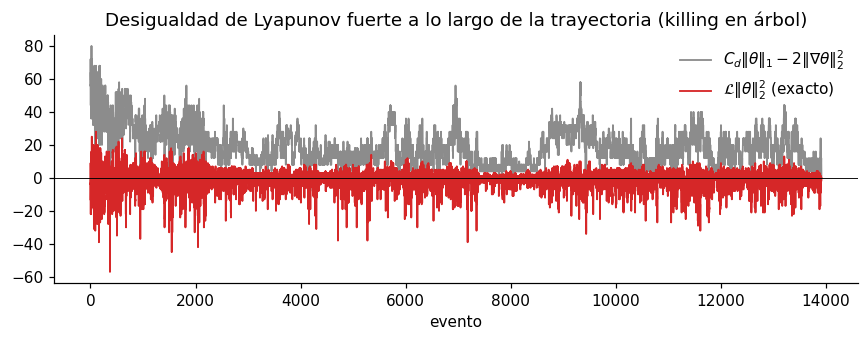
\includegraphics[width=0.85\textwidth]{figuras/lyapunov.png}
\caption{$\Lgen\norm{\theta}_2^2$ exacto (rojo) frente a la cota $C_d\norm{\theta}_1-2\norm{\nabla\theta}_2^2$ (gris) a lo largo de la trayectoria con absorción en el árbol.}
\label{fig:lyapunov}
\end{figure}

\subsection{Poincaré y cantidades conservadas}

\fn{restricted_upper_laplacian} construye $\Delta^{\uparrow}$ restringido a las aristas fuera de $T$, y \fn{poincare_constant} calcula su menor autovalor $c'$ y la dimensión de su núcleo (con álgebra lineal densa, solo para cajas chicas). En la caja $8\times8$:

\begin{center}
\begin{tabular}{@{}lcc@{}}
\toprule
$T$ & $c'$ & $\dim\ker$ \\
\midrule
árbol generador & $0.0127$ & $0$ \\
borde de la caja & $0$ & $49$ (vértices interiores) \\
vacío & $0$ & $80=|V|-1$ \\
\bottomrule
\end{tabular}
\end{center}

Esto es el Lema~2.3 en números: con el árbol, $\norm{\nabla\theta}^2\ge c'\norm{\theta}^2$ con $c'>0$; con el borde de la caja, cada vértice interior $v$ aporta una forma ``invisible'' $\nabla\delta_v$ al núcleo.

\paragraph{Prueba dinámica.} Se coloca \textbf{una sola partícula} en una arista central que no pertenece a ninguno de los dos conjuntos $T$, y se simula con ambos. Con absorción en el borde, la divergencia en los vértices interiores no cambia nunca (desviación máxima $0$, como predice la Proposición~\ref{prop:divergencia}) y el proceso no se extingue. Con el árbol, la divergencia cambia y el proceso se extingue.

%=====================================================================
\section{Visualización}
%=====================================================================

Esta es la sección~5 del notebook. La convención visual es la misma en 2D y en 3D:
\begin{itemize}[nosep]
  \item partículas $+$ en rojo y $-$ en azul;
  \item el proceso de alturas $\eta$ de fondo (en 3D, como placas translúcidas);
  \item el conjunto absorbente $T$ (el árbol generador) en verde pálido;
  \item a la derecha, $\norm{\theta_t}_1$ y las aniquilaciones y absorciones acumuladas.
\end{itemize}

\subsection{Dibujo en dos dimensiones}

\begin{description}[style=nextline, leftmargin=1.2em, font=\normalfont]
  \item[\fn{edge_segments(edges)}] Extremos de cada arista: el baricentro $\pm\frac12$ en su dirección semientera. En coordenadas dobladas basta con $(z-\text{odd})/2$ y $(z+\text{odd})/2$.
  \item[\fn{edge_midpoints}] Baricentros, donde se dibujan los puntos de cada partícula.
  \item[\fn{face_image}] Reacomoda el vector $\eta$ (uno por cara) como imagen: la cara doblada $(2i+1,2j+1)$ va al píxel $(j,i)$.
  \item[\fn{charge_rgba}] Rojo si $\theta_e>0$, azul si $\theta_e<0$, transparente si $\theta_e=0$.
  \item[\fn{draw_lattice_background}] La grilla en gris claro y $T$ en verde pálido, con trazo grueso.
  \item[\fn{init_height_layer}] \fn{imshow} de $\eta$ con un mapa de colores divergente y transparencia.
  \item[\fn{init_particle_layers}, \fn{update_particle_layers}] Un \fn{LineCollection} con todas las aristas coloreadas por carga y un \fn{scatter} con tamaño proporcional a $\sqrt{|\theta_e|}$.
  \item[\fn{init_norm_panel}, \fn{init_counts_panel}] $\norm{\theta_t}_1$ arriba y aniquilaciones y absorciones acumuladas abajo, cada panel con un cursor rojo.
  \item[\fn{build_animation_figure}] Arma la figura con los tres paneles.
  \item[\fn{make_frame_updater}] Crea la función \fn{update(j)} que pide \fn{FuncAnimation}, como \emph{closure} sobre los datos precalculados.
  \item[\fn{animate_process}, \fn{save_animation}, \fn{render_video}, \fn{show_video}] Reconstruir y animar; guardar en MP4 con ffmpeg (o GIF con Pillow si no hay ffmpeg); todo junto cerrando la figura; mostrar el video en el notebook.
\end{description}

\subsection{Dibujo en tres dimensiones}

\begin{description}[style=nextline, leftmargin=1.2em, font=\normalfont]
  \item[\fn{face_polygons}] Las cuatro esquinas de cada cara, $c-a-b,\ c+a-b,\ c+a+b,\ c-a+b$ con $a=\frac12e_i$, $b=\frac12e_j$, en el orden de su borde orientado.
  \item[\fn{box_wireframe_segments}] Las doce aristas del cubo: pares de esquinas que difieren en una sola coordenada.
  \item[\fn{height_rgba}] Colores casi transparentes para las placas de $\eta$.
  \item[\fn{init_3d_axes}] La caja y el árbol $T$ en verde pálido, semitransparente.
  \item[\fn{init_height_layer_3d}, \fn{init_particle_layers_3d} y sus \fn{update}] Igual que en 2D, pero con \fn{Line3DCollection}, \fn{Poly3DCollection} y \fn{scatter} 3D. Solo se dibujan las aristas ocupadas y las caras con $\eta\ne0$, para no saturar la imagen.
  \item[\fn{make_frame_updater_3d}] Además gira lentamente la cámara (\fn{view_init}) para dar sensación de profundidad.
  \item[\fn{planar_face_block_mask}, \fn{planar_loop_configuration}] Un lazo en un plano $z=\text{constante}$; lo usa \fn{init_loop} en 3D.
\end{description}

\noindent Además, \fn{adaptive_fps} y \fn{render_any_dimension} eligen el renderizador 2D o 3D y ajustan los cuadros por segundo, para que los videos duren varios segundos aunque la trayectoria tenga pocos eventos.

\subsection{Qué cambia en \texorpdfstring{$\Z^3$}{Z3}}

\textbf{La simulación no cambia}: todas las funciones aceptan cualquier dimensión $d$. Lo que cambia es la geometría:
\begin{itemize}[nosep]
  \item en el interior $\lambda_e=2(d-1)=4$, porque cada arista toca cuatro caras;
  \item la constante del Teorema~2.1 es $C_3=16$;
  \item un árbol generador tiene $|V|-1$ aristas, que en 3D son solo alrededor del $39\%$ del total (en 2D eran cerca del $50\%$), así que la absorción es proporcionalmente más débil.
\end{itemize}

Las verificaciones en la caja $6^3$ pasan todas: $\partial_1\partial_2=0$, reconstrucción exacta, identidad de conteo, Lyapunov con $C_3=16$, drift con $0.85\%$ de error, y Poincaré con $c'=0.0032>0$ para el árbol y núcleo de dimensión $125=5^3$ (los vértices interiores) para el borde de la caja.

%=====================================================================
\section{Réplicas, condiciones iniciales y absorción}\label{sec:replicas}
%=====================================================================

Esta es la sección~6 del notebook: herramientas comunes a los videos y al estudio de extinción.

\subsection{Réplicas reproducibles en paralelo}

\begin{description}[style=nextline, leftmargin=1.2em, font=\normalfont]
  \item[\fn{replica_seeds(master, n)}] Semillas independientes con \fn{SeedSequence(master).spawn(n)}.
  \item[\fn{simulate_replica(cx, init_fn, kill_fn, seed, ...)}] Una réplica completa con un único generador \fn{rng}, usado en este orden: $\theta_0=$ \fn{init_fn(cx, rng)}, luego $T=$ \fn{kill_fn(cx, theta0, rng)}, y luego la simulación. Como el orden es fijo, la misma semilla reproduce exactamente la misma réplica. Eso es lo que permite elegir una réplica en una búsqueda y volver a simularla para el video.
  \item[\fn{replica_summary}, \fn{replica_chunk}, \fn{run_replicas}] Ejecutan $R$ réplicas repartidas en bloques que corren en paralelo con \fn{joblib}, y devuelven un \fn{ReplicaSample} con $\tau$, el número de eventos, si hubo extinción y el máximo de $\norm{\theta_t}_1$. Cada bloque construye el complejo una sola vez. El resultado no depende del número de núcleos.
  \item[\fn{wilson_interval}] Intervalo de Wilson al 95\,\% para una proporción $\hat p=x/n$:
  \[
  \frac{\hat p+\frac{z^2}{2n}}{1+\frac{z^2}{n}}\;\pm\;\frac{z}{1+\frac{z^2}{n}}\sqrt{\frac{\hat p(1-\hat p)}{n}+\frac{z^2}{4n^2}},\qquad z=1.96.
  \]
  A diferencia del intervalo normal $\hat p\pm z\sqrt{\hat p(1-\hat p)/n}$, no colapsa cuando $\hat p$ es $0$ o $1$, que es justamente donde viven muchas de nuestras probabilidades.
\end{description}

El motor acepta ahora, además de \fn{t_max}, un parámetro \fn{l1_max}: la simulación se corta si $\norm{\theta}_1$ alcanza ese valor. Sirve para medir la extinción \emph{temprana} en 3D, es decir, la extinción antes de escapar a la meseta.

\subsection{Condiciones iniciales y conjuntos absorbentes}

\begin{description}[style=nextline, leftmargin=1.2em, font=\normalfont]
  \item[\fn{init_loop}] El lazo unitario $\theta_0=\partial f$ de la cara central. En 3D es la cara horizontal central. Tiene divergencia nula.
  \item[\fn{init_single_particle}] Una partícula $+1$ en la arista más cercana al centro.
  \item[\fn{init_random_particles(cx, rng, n, radius)}] $n$ partículas $+1$ en aristas uniformes a distancia $\ell^\infty$ a lo más \fn{radius} del centro. Pueden apilarse en una misma arista.
  \item[\fn{kill_none}] $T=\emptyset$.
  \item[\fn{kill_tree}] Árbol generador aleatorio que evita el soporte de $\theta_0$ (ver abajo).
\end{description}

\subsection{El árbol que evita la condición inicial}

Si el árbol pasara por las aristas iniciales, esas partículas morirían en $t=0$. La función \fn{spanning_tree_avoiding_mask(d1, avoid, rng)} asigna a cada arista el peso
\[
w_e=u_e+M\,\mathbf 1_{e\in A},\qquad u_e\sim U(1,2)\ \text{i.i.d.},\qquad M=2|V|,
\]
donde $A$ es el conjunto a evitar, y calcula el árbol generador mínimo.

\begin{proposicion}
El árbol generador mínimo para los pesos $w$ usa el mínimo número posible de aristas de $A$ entre todos los árboles generadores.
\end{proposicion}

\begin{proof}
Todo árbol generador tiene exactamente $|V|-1$ aristas, así que su peso base $\sum_{e\in T}u_e$ está en $[|V|-1,\,2(|V|-1))$. La diferencia de pesos base entre dos árboles es entonces menor que $|V|-1<M$. Si $T_1$ usa menos aristas de $A$ que $T_2$, la penalización de $T_2$ supera a la de $T_1$ en al menos $M$, que es mayor que cualquier diferencia de pesos base. Por lo tanto $w(T_1)<w(T_2)$, y el mínimo se alcanza en un árbol con el menor número de aristas de $A$.
\end{proof}

%=====================================================================
\section{Videos}
%=====================================================================

Esta es la sección~7 del notebook, con seis videos de simulaciones y dos videos extra, \emph{Stochastic Ninja Warrior}, en los que el conjunto absorbente se mueve (\S\ref{sec:ninja}):

\begin{center}
\small
\begin{tabular}{@{}cllll@{}}
\toprule
 & caja & condición inicial & absorción & resultado \\
\midrule
1 & $7\times7$ & lazo $\partial f$ & ninguna & extinción en 91 eventos \\
2 & $7\times7$ & lazo $\partial f$ & árbol generador & extinción en 197 eventos \\
3 & $7\times7$ & 10 partículas $+1$ & árbol generador & extinción en 1\,629 eventos \\
4 & $7\times7\times7$ & 10 partículas $+1$ & árbol generador & meseta ($\approx370$ partículas a los 30\,000 eventos) \\
5 & $3\times3\times3$ & lazo $\partial f$ & árbol generador & extinción en 23\,286\,239 eventos (sin seleccionar) \\
6 & $3\times3\times3$ & 10 partículas $+1$ & árbol generador & extinción en 90\,617\,992 eventos (sin seleccionar) \\
\bottomrule
\end{tabular}
\end{center}

\subsection{Por qué 3D usa dos cajas}

Antes de elegir las cajas se midió cómo termina cada simulación:
\begin{itemize}[nosep]
  \item en $7\times7\times7$ con 10 partículas y árbol, ninguna de 20 réplicas se extinguió en $10^6$ eventos: la simulación muere en unos pocos eventos o crece hasta una meseta de cientos de partículas;
  \item en $4\times4\times4$ con 10 partículas, ninguna de las corridas de prueba se extinguió en $4\cdot10^7$ eventos (meseta de $\approx94$ partículas);
  \item en $3\times3\times3$ la meseta es de $\approx40$ partículas, y de ahí el proceso sí se extingue en unas decenas de millones de eventos.
\end{itemize}
Por eso el video 4 muestra el \textbf{crecimiento y la meseta} en $7\times7\times7$, y los videos 5 y 6 muestran corridas completas \textbf{hasta la extinción} en $3\times3\times3$.

\subsection{La regla de selección (solo en los videos 1 y 2)}

El lazo se extingue muchas veces en el primer evento: si la cara que suena es la misma $f$, entonces $\theta-\partial f=0$. En $7\times7$, una simulación cualquiera daría un video de una fracción de segundo. Por eso, en los videos 1 y 2 se usa una regla fija y explícita (\fn{first_replica_where} con \fn{branched_then_extinct}): entre réplicas con semillas en un orden fijo, se muestra \textbf{la primera que se extingue después de alcanzar 8 partículas}. Esos videos son trayectorias \emph{condicionadas} a ramificarse y después extinguirse, no trayectorias típicas. El notebook reporta que cumplen la condición el 36\,\% de las réplicas sin árbol y el 7\,\% con árbol.

Los videos 3 a 6 usan la \textbf{primera semilla}, sin ninguna selección.

\subsection{Videos 5 y 6: corridas completas hasta la extinción}

En 3D no se elige la trayectoria: se toma la primera semilla y se deja correr la simulación todo lo necesario. Con el lazo y un árbol en $3\times3\times3$, eso fueron 23\,286\,239 eventos (tiempo $t\approx3.2\cdot10^{5}$), con un máximo de 41 partículas. Casi toda la corrida transcurre en la meseta, entre 10 y 40 partículas. La extinción llega de golpe: la última foto antes del final todavía tenía 33 partículas, y el proceso se extinguió en menos de 32\,768 eventos, es decir, en el último 0.15\,\% de la corrida. Es lo típico de un régimen cuasi-estacionario: la salida de la meseta es un evento raro pero rápido. Como referencia, con la misma semilla el lazo \emph{sin} árbol se extingue en el primer evento, así que no hay nada que mostrar en ese caso.

El video 6 repite el experimento partiendo de 10 partículas $+1$, también con la primera semilla: es la corrida ``honesta'' de cuánto puede tardar la extinción en 3D. Tardó \textbf{90\,617\,992 eventos} (tiempo $t\approx1.1\cdot10^{6}$, máximo de 44 partículas), con 10.2 minutos de cómputo, frente a 2.6 minutos del video 5. El notebook imprime al final una tabla con los tiempos reales de ambas corridas (\S\ref{sec:fund-largas}).

\paragraph{Fotos con adelgazamiento} (\fn{run_until_extinction}). Guardar cada evento de una corrida de decenas de millones de eventos no es razonable, y tampoco se sabe de antemano cuánto va a durar. El motor guarda \emph{fotos} $(n,t,\theta)$:
\begin{itemize}[nosep]
  \item una foto cada \fn{every} eventos, empezando con \fn{every} $=1$;
  \item cuando se juntan $2N$ fotos ($N=400$), se descarta una de cada dos y se duplica \fn{every}.
\end{itemize}
Después de cada adelgazamiento las fotos restantes siguen equiespaciadas (los múltiplos de $2\,\fn{every}$ son la mitad de los múltiplos de \fn{every}). Por lo tanto, al final hay entre $N$ y $2N$ fotos equiespaciadas en número de eventos, \textbf{cualquiera sea la duración}, y la memoria nunca supera $2N$ fotos. En el video 5 quedaron 712 fotos, una cada 32\,768 eventos; en el video 6, 693 fotos, una cada 131\,072 eventos.

\paragraph{El video} (\fn{animate_snapshots_3d}). Muestra todas las fotos, así que es la corrida completa en cámara rápida: cada cuadro avanza 32\,768 eventos en el video 5 y 131\,072 en el video 6. El muestreo ponderado de la arista usa inversión de la distribución acumulada (\fn{cumsum} y \fn{searchsorted}), que en corridas tan largas es más rápido que \fn{rng.choice}: unos $10\,\mu$s por evento.

\begin{figure}[ht]
\centering
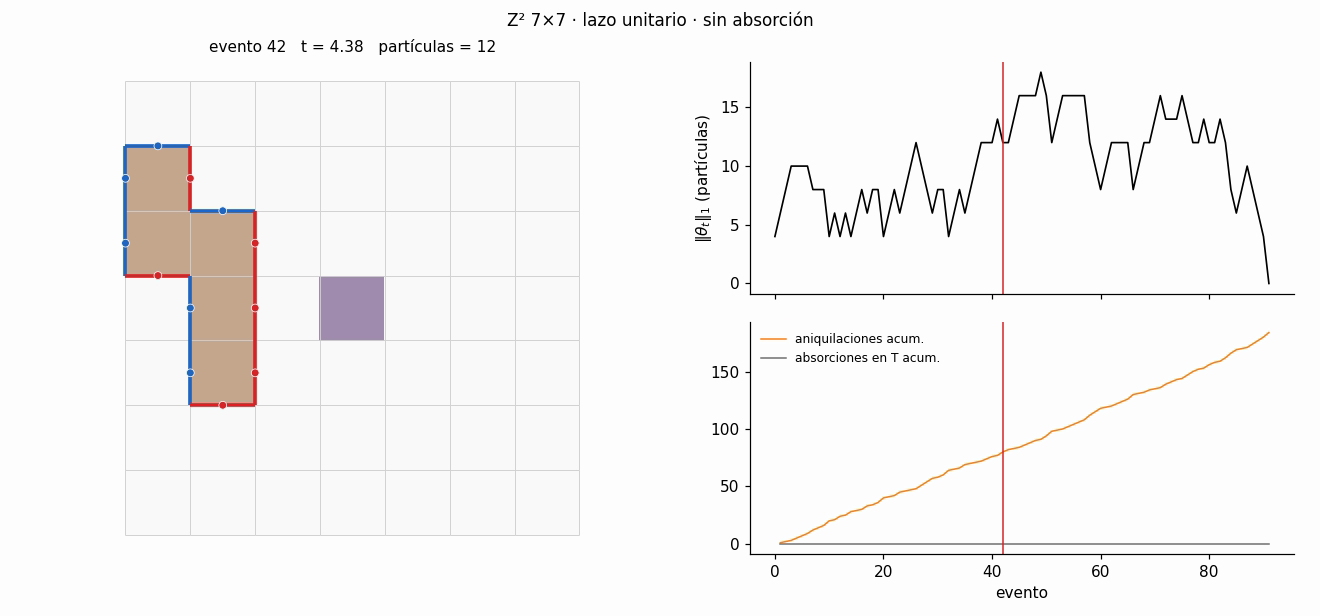
\includegraphics[width=0.49\textwidth]{figuras/vid_z2_lazo_sin_arbol.png}\hfill
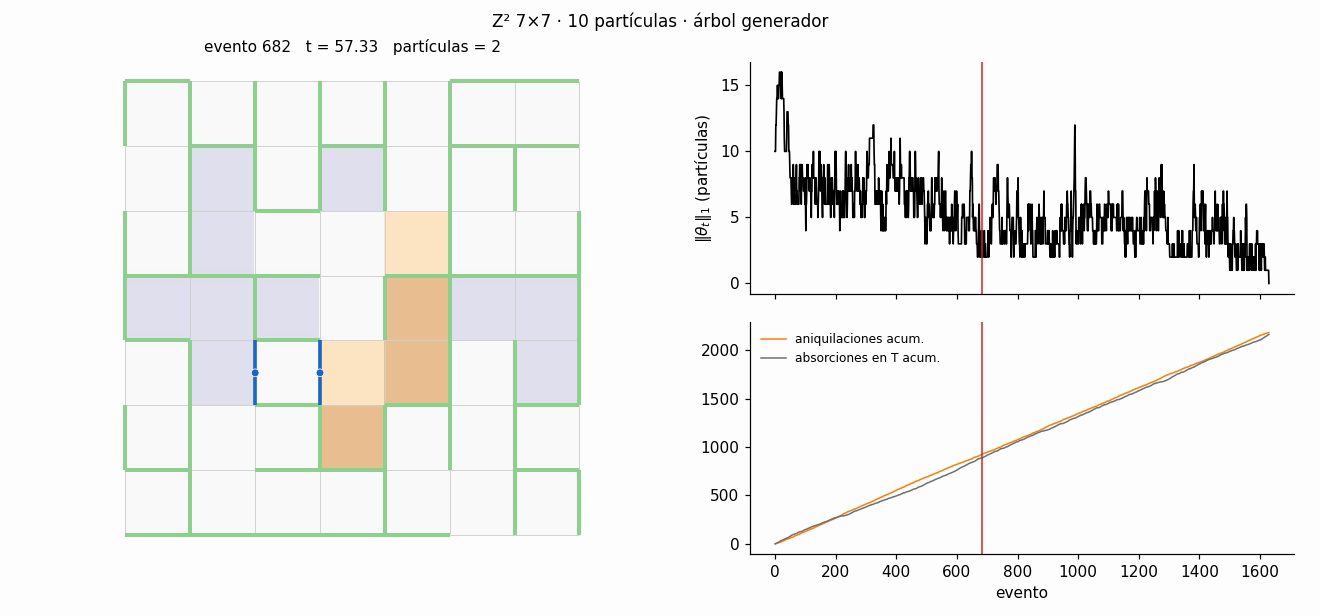
\includegraphics[width=0.49\textwidth]{figuras/vid_z2_10particulas.png}\\[2mm]
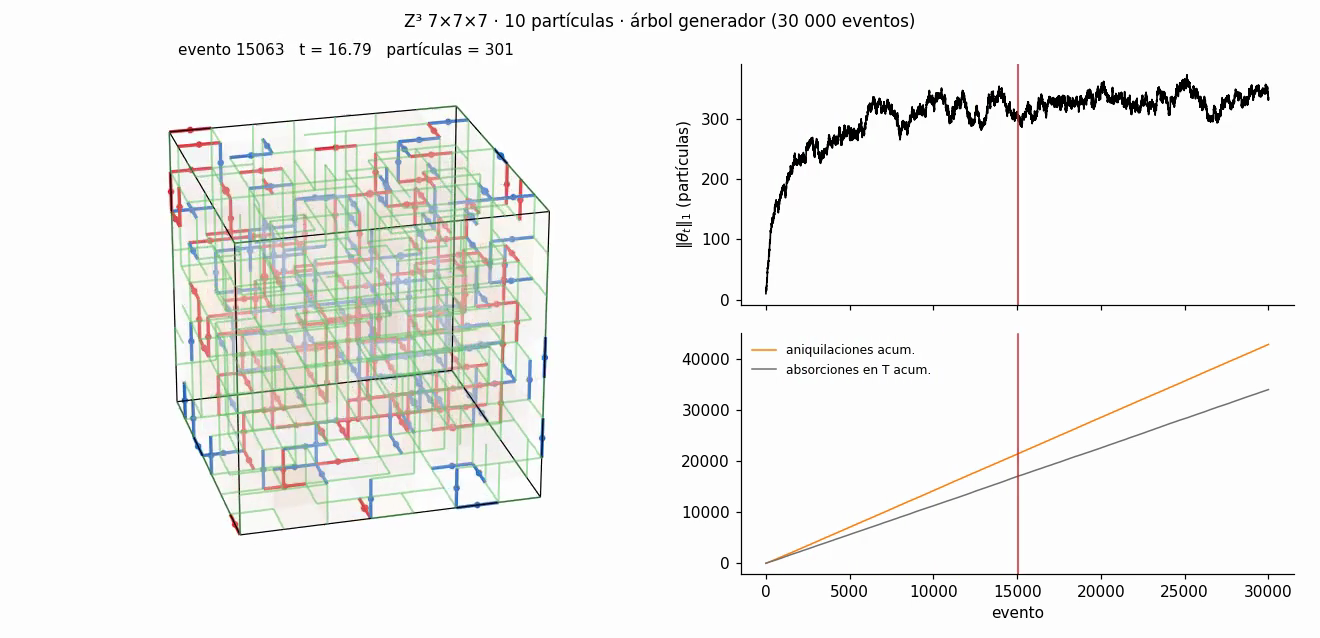
\includegraphics[width=0.49\textwidth]{figuras/vid_z3_meseta.png}\hfill
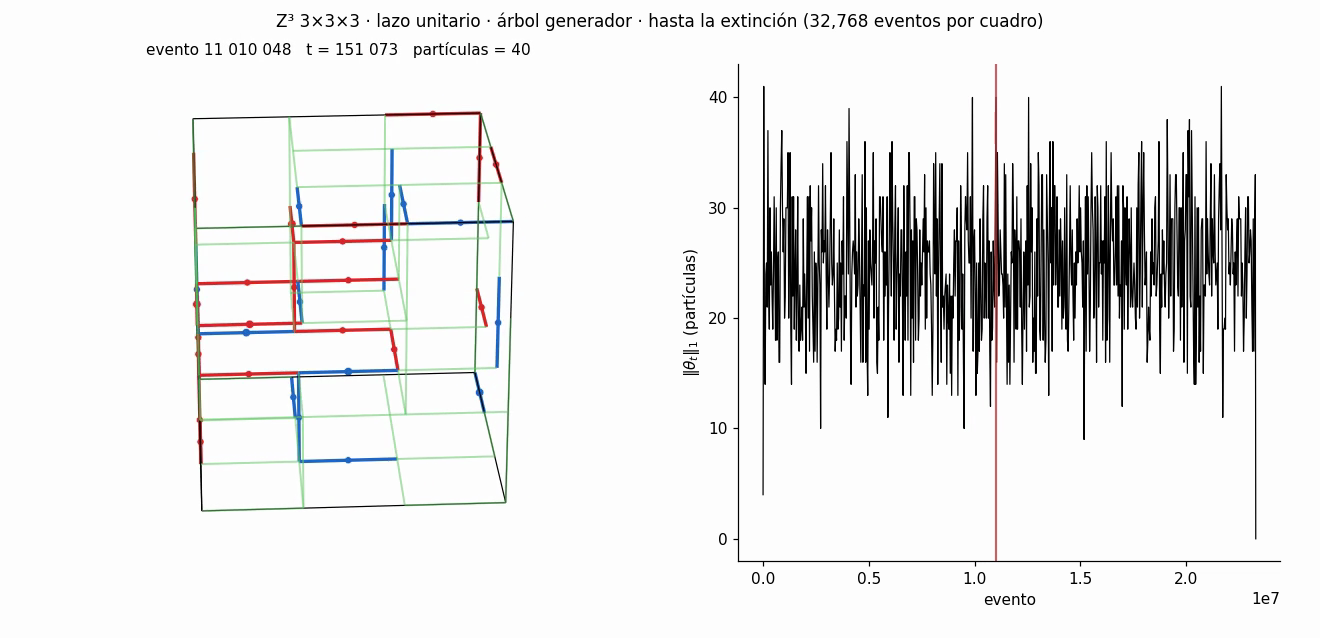
\includegraphics[width=0.49\textwidth]{figuras/vid_z3_lazo_con_arbol.png}
\caption{Cuadros de los videos 1 (arriba izquierda), 3 (arriba derecha), 4 (abajo izquierda) y 5 (abajo derecha). En el video 1 las partículas forman la frontera de las regiones del proceso de alturas $\eta$, porque $\theta_t=\theta_0+\partial\eta_t$ y $\theta_0$ es un borde.}
\label{fig:videos}
\end{figure}


\begin{figure}[ht]
\centering
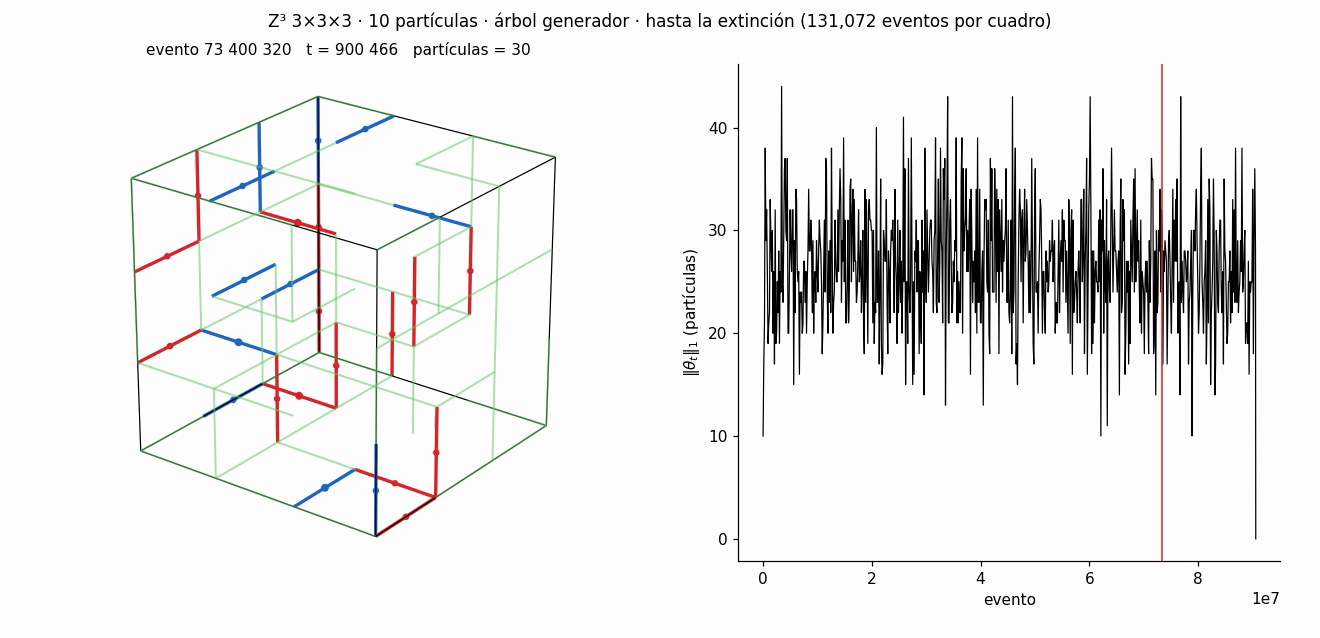
\includegraphics[width=0.85\textwidth]{figuras/vid_z3_10particulas_extincion.png}
\caption{Video 6: $\Z^3$, caja $3\times3\times3$, 10 partículas y árbol, corrido hasta la extinción sin selección (90\,617\,992 eventos). A la derecha, la cantidad de partículas en toda la corrida: meseta durante casi todo el tiempo y extinción al final.}
\label{fig:video6}
\end{figure}

\subsection{Videos 7 y 8: \emph{Stochastic Ninja Warrior}}\label{sec:ninja}

Ocho partículas $+1$ (los ``concursantes'') parten en aristas distintas elegidas al azar y evolucionan con la dinámica de siempre. La diferencia es que el conjunto absorbente es un \textbf{obstáculo que se mueve}: $T=T(t)$ depende del tiempo y elimina a toda partícula que toca. Hay dos pruebas, cada una de 3 ciclos de período 12:

\paragraph{La cruz giratoria} (caja $14\times14$). $T(t)$ son cuatro brazos de radio 6 que salen del vértice central en los ángulos $2\pi t/12+q\frac{\pi}{2}$, con $q=0,1,2,3$.
\begin{description}[style=nextline, leftmargin=1.2em, font=\normalfont]
  \item[\fn{lattice_path_ray(center, angle, radius)}] Versión 4-conexa del algoritmo de Bresenham. En cada paso se elige, entre el movimiento horizontal y el vertical en el sentido del rayo, el que deja el vértice más cerca del rayo. La distancia de un vértice $v$ al rayo de dirección $u$ es $|(v-c)\times u|$.
  \item[\fn{path_edges}, \fn{plus_mask}] Convierten los cuatro caminos en una máscara de aristas: el paso $a\to b$ es la arista con baricentro doblado $a+b$.
\end{description}

\paragraph{El anillo que oscila} (caja $15\times15$). $T(t)$ es el soporte de $\partial_2\big(\text{disco}(r(t))\big)$, con
\[
r(t)=6.5\,\frac{1+\cos(2\pi t/12)}{2},
\]
donde $\text{disco}(r)$ son las caras con baricentro a distancia $\le r$ del centro (\fn{disk_faces}, \fn{ring_mask}). Con $r=0$ el disco es una sola cara y el anillo es exactamente el lazo unitario $\partial f$; el notebook lo verifica. Como el anillo nunca llega a las esquinas, ahí hay ``zonas seguras''.

\paragraph{Simulación exacta con obstáculo móvil} (\fn{run_moving_obstacle}). El obstáculo se discretiza en 720 posiciones por ciclo (\fn{obstacle_table}).
\begin{itemize}[nosep]
  \item En cada evento, las cargas que caen sobre $T(t)$ mueren, igual que con un conjunto absorbente fijo.
  \item Entre eventos las partículas no se mueven. Cuando el reloj avanza de $t$ a $t'$, el obstáculo pasa por todas sus posiciones intermedias, y en cada una elimina a las partículas que encuentra. Así el obstáculo no ``salta por encima'' de nadie, aunque haya pocas partículas y los tiempos entre eventos sean largos.
  \item El estado se guarda directamente en los tiempos de los cuadros, porque con $T$ variable ya no sirve la reconstrucción $\theta_t=\theta_0+\partial_T\eta_t$.
\end{itemize}
Con un $T$ que cambia, las cargas de la Proposición~\ref{prop:cargas} dejan de conservarse, así que la extinción es posible. Aun así, en las pruebas el obstáculo no alcanza a eliminar a todos: la población se estabiliza en unas decenas de partículas, en equilibrio entre la ramificación y las eliminaciones.

\paragraph{El video} (\fn{animate_ninja}, \fn{render_ninja}, \fn{play_ninja}). Muestra el obstáculo en verde, las partículas, una $\times$ naranja en cada arista donde murió una partícula desde el cuadro anterior, y un marcador con las partículas ``en carrera'' y ``eliminadas''. Si no queda nadie, termina con \emph{GAME OVER}. Se usa la primera semilla, sin elegir la trayectoria, y se guarda en MP4 y GIF.

\begin{figure}[ht]
\centering
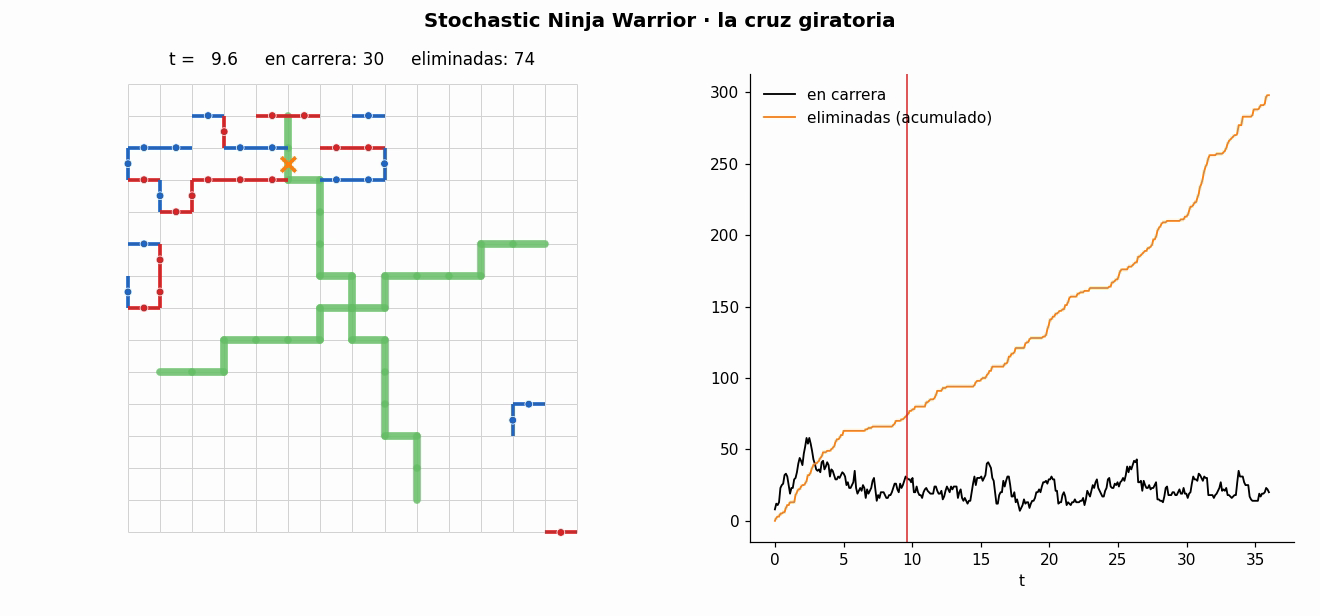
\includegraphics[width=0.49\textwidth]{figuras/ninja_cruz.png}\hfill
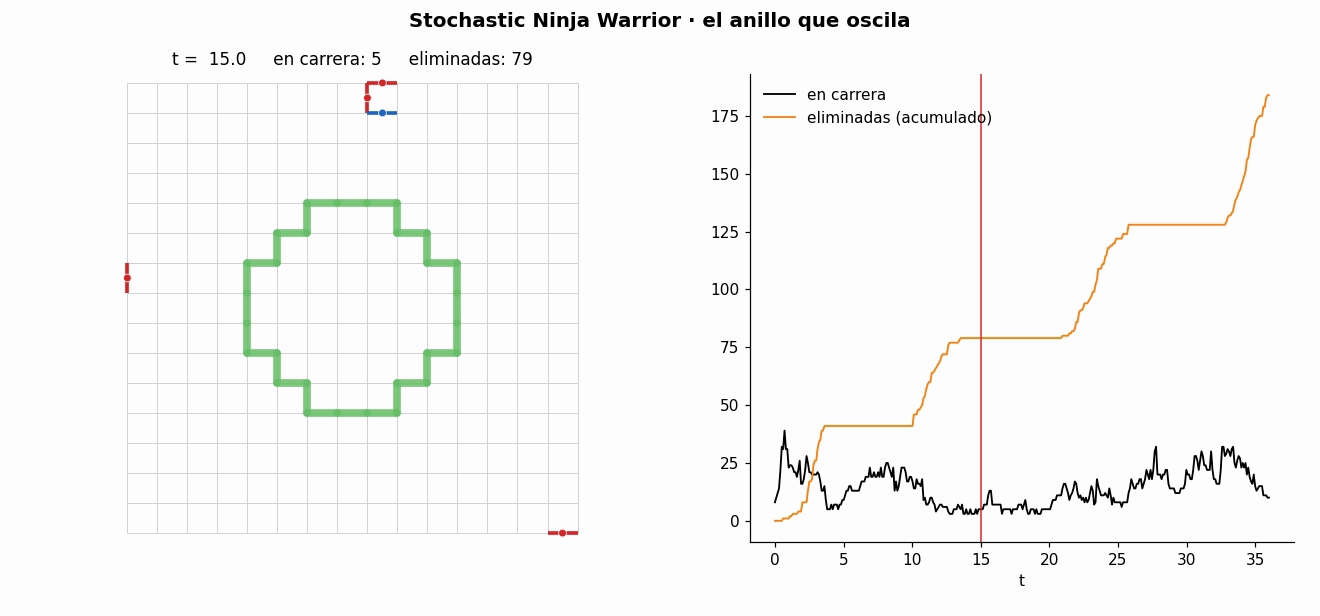
\includegraphics[width=0.49\textwidth]{figuras/ninja_anillo.png}
\caption{\emph{Stochastic Ninja Warrior}: la cruz giratoria (izquierda) y el anillo que oscila (derecha). El obstáculo, en verde, es el conjunto absorbente $T(t)$; las $\times$ naranjas marcan partículas recién eliminadas.}
\label{fig:ninja}
\end{figure}

\subsection{La meseta cuasi-estacionaria en \texorpdfstring{$\Z^3$}{Z3}}

\begin{observacion}
La meseta no contradice el Teorema~2.4. La deriva
\[
\Lgen\norm{\theta}_2^2\le c\norm{\theta}_2-c'\norm{\theta}_2^2
\]
solo empuja hacia abajo cuando $\norm{\theta}_2>c/c'$, y en 3D la constante de Poincaré es diminuta ($c'\approx0.003$ ya en la caja $6^3$). La extinción sigue ocurriendo casi seguramente, pero requiere una fluctuación grande desde la meseta: es un régimen \emph{cuasi-estacionario}, en el que el tiempo de extinción puede crecer muy rápido con el tamaño de la caja.
\end{observacion}

%=====================================================================
\section{Probabilidad de extinción según el número de aristas absorbentes}\label{sec:aristas}
%=====================================================================

Esta es la sección~8 del notebook. Estudia cómo cambia la extinción al ir agregando aristas al conjunto absorbente $T$, desde $T=\emptyset$ hasta un árbol generador, en cajas $9\times9$ y $9\times9\times9$.

\subsection{Cargas conservadas}

Sea $T\subseteq E$ el conjunto absorbente y sean $\mathcal C(T)$ las componentes conexas del grafo $(V,T)$. Un vértice que no toca $T$ forma su propia componente. Para $C\in\mathcal C(T)$ se define la \textbf{carga}
\[
Q_C(\theta)=\sum_{v\in C}(\partial_1\theta)(v),
\]
que es el flujo neto de $\theta$ que sale de $C$. Las aristas internas de $C$ aportan $+1$ y $-1$ dentro de $C$, así que se cancelan.

\begin{proposicion}[Conservación de las cargas]\label{prop:cargas}
Para toda $C\in\mathcal C(T)$, $Q_C(\theta_t)$ es constante en el tiempo. Además, $Q_C(P_T\theta_0)=Q_C(\theta_0)$: matar en $t=0$ las partículas que están sobre $T$ no cambia las cargas.
\end{proposicion}

\begin{proof}
\textit{Un evento.} En un evento,
\[
\theta_{\text{nuevo}}=\theta-c\,P_T\partial f=\theta-c\,\partial f+c\,(I-P_T)\partial f .
\]
El término $-c\,\partial f$ no cambia ninguna divergencia, porque $\partial_1\partial_2=0$.

\noindent\textit{Lo que se descarta.} El término $(I-P_T)\partial f$ está soportado en aristas $e=(u,w)\in T$, y $\partial_1e=w-u$. Como $u$ y $w$ están en la misma componente de $(V,T)$, la contribución de $e$ a $\sum_{v\in C}(\partial_1\,\cdot\,)(v)$ es $1-1=0$ si $u,w\in C$, y $0$ si no. El mismo argumento vale para $(I-P_T)\theta_0$.
\end{proof}

\begin{corolario}[Imposibilidad]\label{cor:imposible}
Si existe $C\in\mathcal C(T)$ con $Q_C(\theta_0)\neq0$, entonces $\theta_t\neq0$ para todo $t$: la extinción es imposible.
\end{corolario}

\begin{proof}
$Q_C(0)=0\ne Q_C(\theta_0)=Q_C(\theta_t)$.
\end{proof}

\noindent La Proposición~\ref{prop:divergencia} (conservación de la divergencia en vértices que no tocan $T$) es el caso de las componentes de un solo vértice.

\begin{proposicion}[Las cargas son la única obstrucción del drift]\label{prop:inyectivo}
Sea $W_T=\{\theta\in\R^{E}:\ \theta|_T=0,\ Q_C(\theta)=0\ \forall C\in\mathcal C(T)\}$. Si $\theta\in W_T$ y $\partial_2^T\theta=0$, entonces $\theta=0$. En consecuencia,
\[
c_W(T)=\min_{\theta\in W_T,\ \norm{\theta}=1}\norm{\partial_2^T\theta}^2>0 .
\]
\end{proposicion}

\begin{proof}
\textit{La forma es un gradiente.} Si $\partial_2^T\theta=0$, la forma $\theta$ es cerrada. Como la caja es simplemente conexa, $\theta=\nabla g=\partial_1^Tg$ para alguna $g:V\to\R$.

\noindent\textit{$g$ es constante por componentes.} Como $\theta|_T=0$, se tiene $g(u)=g(w)$ para toda arista $(u,w)\in T$, así que $g=\sum_{C}a_C\mathbf 1_C$.

\noindent\textit{Las cargas fuerzan $g$ constante.} Con $L=\partial_1\partial_1^T$ el Laplaciano del grafo de la caja, $Q_C(\nabla g)=\mathbf 1_C^TL\,g$. Si $M$ es la matriz de indicadores de las componentes ($V\times\mathcal C$), el vector de cargas es $M^TLM\,a$, donde $M^TLM$ es el Laplaciano del grafo cociente que resulta de contraer cada componente. El grafo de la caja es conexo, así que el cociente también lo es, y su Laplaciano solo anula las constantes. Por lo tanto, cargas nulas implican $a$ constante, $g$ constante y $\theta=0$.

\noindent\textit{La constante.} $W_T$ es un subespacio de dimensión finita en el que $\theta\mapsto\norm{\partial_2^T\theta}$ no se anula fuera del origen, así que su mínimo en la esfera unitaria es positivo.
\end{proof}

\noindent\textbf{Consecuencia.} Si todas las cargas iniciales son nulas, el proceso vive en $W_T$ para siempre: $\theta|_T=0$ por la absorción, y las cargas se conservan. En $W_T$ se cumple $\partial_T^T\theta=\partial_2^T\theta$, así que el Teorema~2.1 da
\[
\Lgen\norm{\theta}_2^2\le C_d\norm{\theta}_1-2c_W(T)\norm{\theta}_2^2\le C_d\sqrt{|E|}\,\norm{\theta}_2-2c_W(T)\norm{\theta}_2^2 ,
\]
que es una deriva geométrica fuera de una bola. Igual que en el Teorema~2.4 del paper, esto da extinción casi segura \emph{suponiendo que desde cualquier estado alcanzable se llega a $0$ con probabilidad positiva}. Esa hipótesis de accesibilidad no la demostramos; las simulaciones la respaldan.

\begin{proposicion}[Monotonía de la extinción eventual]\label{prop:monotonia}
Si $T\subseteq T'$ y todas las cargas de $\theta_0$ respecto de $\mathcal C(T)$ son nulas, también lo son respecto de $\mathcal C(T')$. Por lo tanto, ``la extinción es posible'' es una propiedad monótona creciente en $T$.
\end{proposicion}

\begin{proof}
Cada componente de $(V,T')$ es unión de componentes de $(V,T)$, y la carga es aditiva: $Q_{C_1\cup C_2}=Q_{C_1}+Q_{C_2}$ para componentes disjuntas.
\end{proof}

\paragraph{Casos particulares.}
\begin{itemize}
  \item \textbf{Una partícula} sobre $e_0=(u,w)$: $\partial_1\theta_0=\delta_w-\delta_u$, así que las cargas se anulan si y solo si $u$ y $w$ están en la misma componente. La extinción eventual equivale a que \textbf{$u$ y $w$ estén conectados por aristas de $T$}. Es un problema de conectividad, del tipo percolación.
  \item \textbf{El lazo} $\partial f$, y en general cualquier $\theta_0$ con $\partial_1\theta_0=0$, tiene todas las cargas nulas para cualquier $T$. Se extingue incluso con $T=\emptyset$; en ese caso $W_\emptyset=\ker\partial_1=\operatorname{Im}\partial_2$.
  \item \textbf{$T$ árbol generador}, el caso del paper: hay una sola componente, y su carga $\sum_v(\partial_1\theta)(v)$ es siempre $0$.
\end{itemize}

\paragraph{Verificación.} En la caja $9\times9$, con $T$ formado por $k$ aristas uniformes y una partícula, se simularon 300 réplicas por cada $k\in\{0,20,\dots,140\}$ (\fn{check_charge_prediction}). Las réplicas en que la extinción es posible se simulan hasta $3\cdot10^5$ eventos, y las demás hasta $2\cdot10^4$. La función \fn{plot_prediction_check} muestra el resultado (figura~\ref{fig:verificacion}):
\begin{itemize}[nosep]
  \item a la izquierda, la proporción de réplicas en que la extinción es posible según las cargas, junto a la proporción que efectivamente se extinguió; las dos curvas coinciden para todo $k$;
  \item a la derecha, la matriz predicción $\times$ observación de las 2400 réplicas: solo la diagonal tiene réplicas. \textbf{Ninguna} réplica ``imposible'' se extinguió y \textbf{todas} las ``posibles'' se extinguieron.
\end{itemize}

\begin{figure}[ht]
\centering
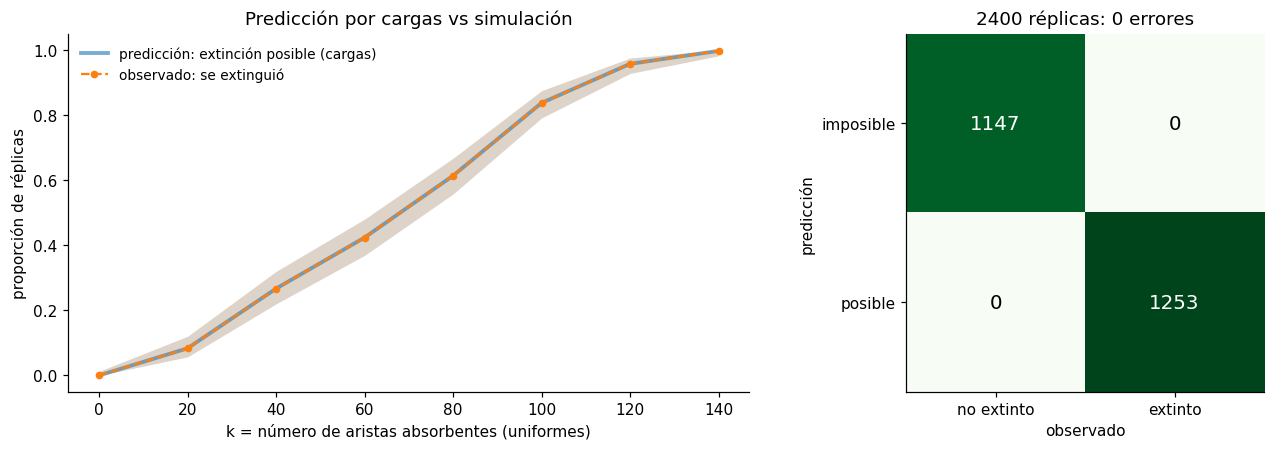
\includegraphics[width=\textwidth]{figuras/verificacion_cargas.png}
\caption{Verificación de la Proposición~\ref{prop:cargas} y el Corolario~\ref{cor:imposible}: predicción por cargas contra simulación, con bandas de Wilson al 95\,\%, y matriz de confusión.}
\label{fig:verificacion}
\end{figure}

\subsection{Reglas para agregar aristas}

Una regla produce un orden de aristas $e_1,e_2,\dots$ y la familia creciente $T_k=\{e_1,\dots,e_k\}$:
\begin{description}[style=nextline, leftmargin=1.2em, font=\normalfont]
  \item[uniforme (\fn{order_uniform})] Orden aleatorio de todas las aristas. Llega a ser generador recién cerca de $|E|$.
  \item[árbol aleatorio (\fn{order_random_tree})] Tipo Kruskal: se recorren las aristas en orden aleatorio y se acepta una solo si une dos componentes distintas. Termina exactamente en un árbol generador en $k=|V|-1$.
  \item[BFS desde el centro (\fn{order_bfs_tree})] El árbol de búsqueda en anchura desde el vértice central, en orden de descubrimiento de los vértices. Las aristas absorbentes empiezan cerca de la condición inicial. Una versión desde una esquina se probó y se descartó, porque no aportaba información nueva.
\end{description}
Las reglas no evitan la condición inicial: las partículas que caen en $T_k$ mueren en $t=0$. Por eso la regla BFS desde el centro mata a una partícula central casi de inmediato.

\subsection{Cálculo exacto de la probabilidad eventual}

Dados un orden y $\theta_0$, sea $k^\ast$ el menor $k$ tal que todas las cargas de $(V,T_k)$ son nulas. Por las Proposiciones~\ref{prop:cargas}--\ref{prop:monotonia},
\[
\mathbb{P}(\tau<\infty\mid T_k,\theta_0)=\mathbf 1\{k^\ast\le k\},\qquad\text{y entonces}\qquad \mathbb{P}(\tau<\infty\mid k)=\mathbb{P}(k^\ast\le k),
\]
la función de distribución de $k^\ast$. La dirección ``$=0$ si $k<k^\ast$'' es rigurosa (Corolario~\ref{cor:imposible}); la dirección ``$=1$'' usa la hipótesis de accesibilidad.

La función \fn{extinction_threshold} calcula $k^\ast$ en una pasada sobre el orden, con una estructura \emph{union--find}: cada componente guarda su carga, y se lleva la cuenta de cuántas componentes tienen carga no nula. Al agregar una arista que une dos componentes, se suman sus cargas y se actualiza el contador; $k^\ast$ es el primer $k$ en que el contador llega a $0$. El costo es casi lineal en $|E|$ y no requiere simular el proceso, así que se pueden usar miles de muestras de $(\theta_0,\text{orden})$ (\fn{sample_thresholds}).

\subsection{Resultados en \texorpdfstring{$\Z^2$}{Z2}: probabilidad eventual}

Con 5000 muestras por regla y condición inicial (figura~\ref{fig:aristas-exacta}):
\begin{itemize}
  \item \textbf{Una partícula.}
  \begin{itemize}[nosep]
    \item Las reglas uniforme y árbol aleatorio coinciden hasta $k\approx60$, con $\mathbb{P}(\tau<\infty)$ creciendo casi linealmente.
    \item El árbol aleatorio llega a 1 en $k=|V|-1=99$, por construcción. Con la regla uniforme, en ese mismo $k$ la probabilidad es solo $0.83$, y hacen falta $\approx150$ aristas para llegar a 1.
    \item BFS desde el centro vale 1 casi desde el comienzo ($k=3$), porque absorbe de inmediato la arista de la partícula.
  \end{itemize}
  \item \textbf{Diez partículas $+1$.} Hacen falta más aristas: la mediana de $k^\ast$ es 92 con árbol aleatorio y 106 con la regla uniforme, donde $\mathbb{P}(k^\ast\le99)=0.31$. Las curvas BFS tienen escalones, porque el árbol neutraliza grupos de partículas a la vez.
  \item \textbf{Lazo.} $\mathbb{P}(\tau<\infty)=1$ para todo $k$.
\end{itemize}

\begin{figure}[ht]
\centering
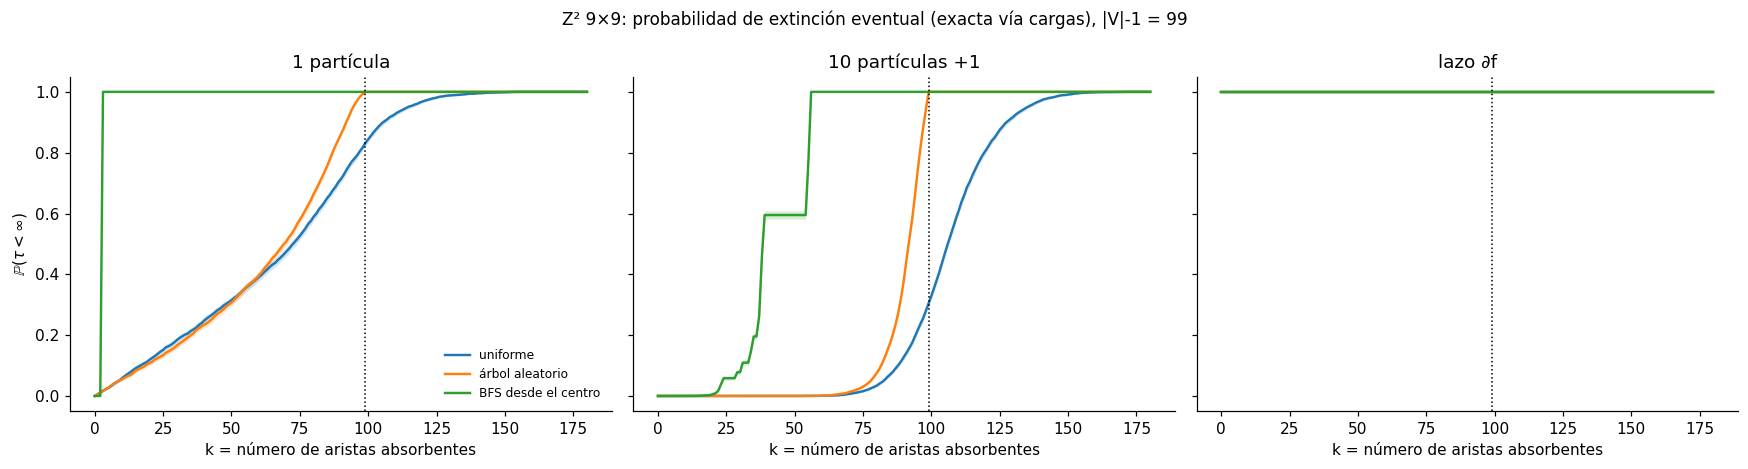
\includegraphics[width=\textwidth]{figuras/aristas_exacta.png}
\caption{$\Z^2$, caja $9\times9$: probabilidad de extinción eventual, exacta vía cargas, en función del número de aristas absorbentes, para cuatro reglas. La línea punteada marca $k=|V|-1$.}
\label{fig:aristas-exacta}
\end{figure}

\subsection{Resultados en \texorpdfstring{$\Z^2$}{Z2}: extinción en tiempo finito}

Que la extinción sea posible no dice cuánto tarda. El notebook mide $\mathbb{P}(\tau\le t^\ast)$ con $t^\ast=50$, con 1000 réplicas por punto y bandas de Wilson (figura~\ref{fig:aristas-finito}). Siempre $\mathbb{P}(\tau\le t^\ast)\le\mathbb{P}(\tau<\infty)$.

\begin{itemize}
  \item \textbf{Una partícula, reglas uniforme y árbol aleatorio:} $\mathbb{P}(\tau\le50)$ sigue de cerca la cota exacta. Una vez que la extinción es posible, ocurre rápido.
  \item \textbf{Lazo:} $\mathbb{P}(\tau\le50)$ \textbf{baja} de $1.00$ ($T=\emptyset$) a $0.94$ con un árbol generador completo: agregar aristas absorbentes hace más lenta la extinción. Con la regla uniforme baja hasta $\approx0.977$ y vuelve a $1$ cuando $T$ cubre las aristas del lazo, que entonces muere en $t=0$.
\end{itemize}

\noindent La extinción en tiempo finito \textbf{no es monótona} en $T$, aunque la eventual sí lo sea. Esto ya se veía en un experimento previo en $5\times5$ con el lazo: con $T$ igual al borde de la caja, la probabilidad de sobrevivir más de 200 eventos era 16 veces la de $T=\emptyset$.

\noindent\textit{Mecanismo (hipótesis).} Sin absorción, un lazo cerrado puede desaparecer por sí solo, por aniquilación. Matar partículas lo corta en cadenas abiertas cuyos extremos llevan carga, y esas cadenas solo desaparecen al llegar a $T$.

\begin{figure}[ht]
\centering
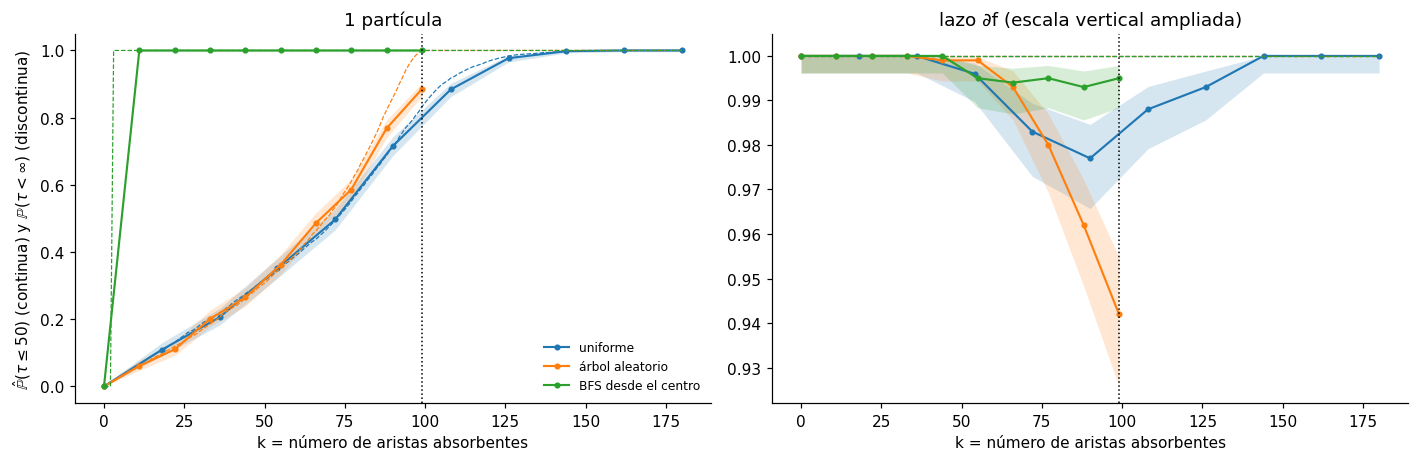
\includegraphics[width=\textwidth]{figuras/aristas_tiempo_finito.png}
\caption{$\hat{\mathbb{P}}(\tau\le50)$ en función de $k$, con banda de Wilson al 95\,\% (línea continua), y la probabilidad eventual exacta (línea discontinua). En el panel del lazo la escala vertical está ampliada.}
\label{fig:aristas-finito}
\end{figure}

\subsection{\texorpdfstring{$T$}{T} creciendo durante la simulación}

En \fn{run_growing_absorption}, $T$ parte vacío y, antes de los eventos número $0,m,2m,\dots$, se agrega la siguiente arista del orden. Las partículas que estén sobre ella mueren en ese momento. Esto sigue hasta completar el orden, que para las reglas de árbol es un árbol generador; desde ahí la extinción está garantizada. Se miden $\mathbb{E}[\tau]$ y $\mathbb{P}(\tau\le50)$ en función de $m$, con 600 réplicas por punto (figura~\ref{fig:aristas-dinamico}).

\begin{itemize}
  \item \textbf{Una partícula:} que $T$ crezca más rápido acelera la extinción. Con árbol aleatorio, $\mathbb{E}[\tau]=69$ con $m=1$ frente a $432$ con $m=100$.
  \item \textbf{Lazo:} ocurre lo contrario. $\mathbb{E}[\tau]=9.7$ con $m=1$ frente a $1.1$ con $m=100$. Si $T$ crece lento, el lazo alcanza a aniquilarse solo antes de que el árbol lo corte.
\end{itemize}

\begin{figure}[ht]
\centering
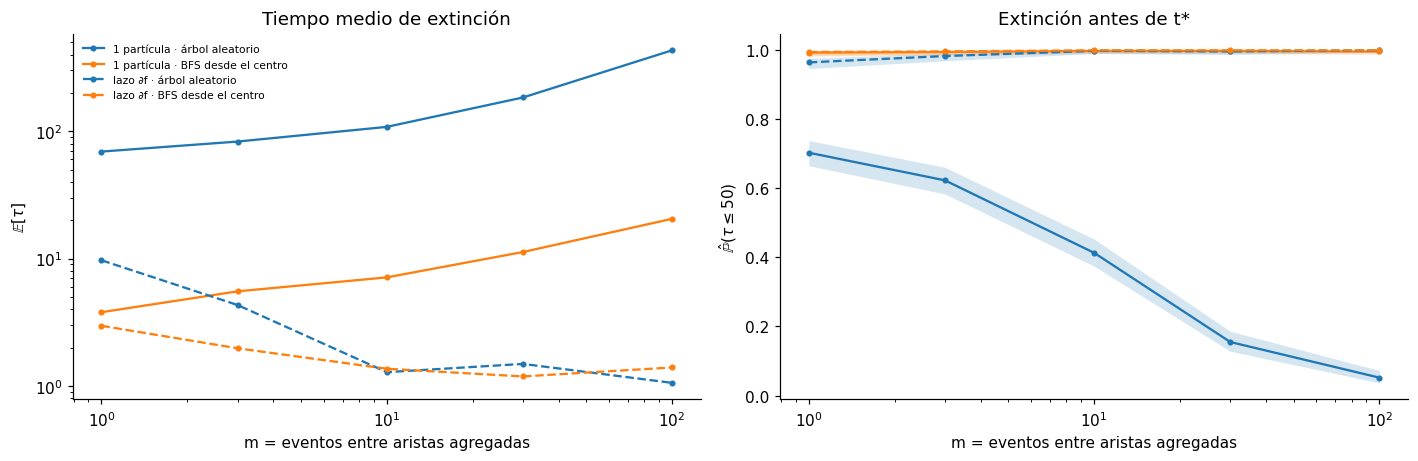
\includegraphics[width=\textwidth]{figuras/aristas_dinamico.png}
\caption{$T$ creciendo durante la simulación: tiempo medio de extinción y $\hat{\mathbb{P}}(\tau\le50)$ en función de $m$ (eventos entre aristas agregadas). Línea continua: una partícula; discontinua: lazo.}
\label{fig:aristas-dinamico}
\end{figure}

\subsection{Resultados en \texorpdfstring{$\Z^3$}{Z3}}

En la caja $9\times9\times9$ la extinción eventual sigue estando dada por las cargas, pero en la práctica casi nunca se observa. Por eso se compara con la probabilidad de \textbf{extinción temprana}
\[
q_M=\mathbb{P}\big(\text{extinción antes de alcanzar }\norm{\theta}_1=M\big),\qquad M=100,
\]
estimada con \fn{l1_max} y 600 réplicas por punto (figura~\ref{fig:aristas-3d}).

\begin{itemize}
  \item \textbf{Una partícula:} $q_{100}$ sigue a $\mathbb{P}(\tau<\infty)$ para $k$ chico. Con las reglas de árbol, en cambio, se queda en $\approx0.3$--$0.4$ aun cuando la extinción eventual es segura: el resto escapa a la meseta.
  \item \textbf{Lazo:} $q_{100}\approx0.33$ para todo $k$ con las reglas de árbol. Su extinción temprana es la autoaniquilación de los primeros eventos, en la que $T$ no influye.
  \item \textbf{Regla uniforme:} $q_{100}\to1$ solo cuando $T$ cubre la mayoría de las aristas ($k\gtrsim1700$ de $2700$).
\end{itemize}

\begin{figure}[ht]
\centering
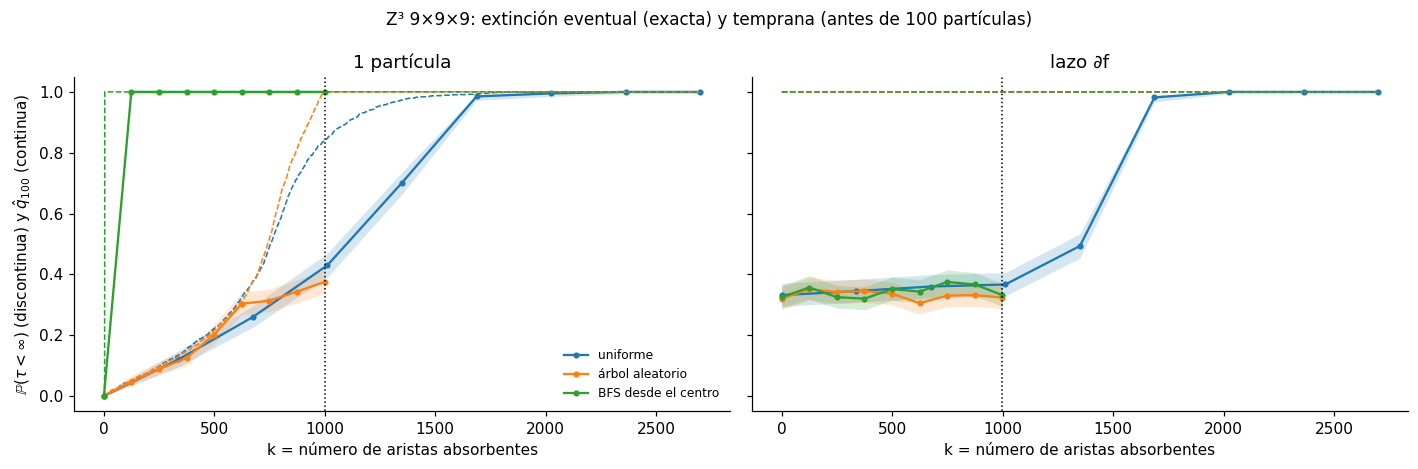
\includegraphics[width=\textwidth]{figuras/aristas_3d.png}
\caption{$\Z^3$, caja $9\times9\times9$: extinción eventual exacta (línea discontinua) y extinción temprana $\hat q_{100}$ con banda de Wilson (línea continua).}
\label{fig:aristas-3d}
\end{figure}

\subsection{Resumen}

\begin{enumerate}
  \item Las cargas $Q_C$ de las componentes de $(V,T)$ se conservan y deciden si la extinción es posible. La probabilidad de extinción eventual es una probabilidad de conectividad, se calcula exactamente y es monótona en $T$.
  \item La extinción en tiempo finito no es monótona en $T$: para el lazo, absorber más, o absorber antes, la hace más lenta.
  \item Con $T$ creciendo durante la simulación, la velocidad de crecimiento tiene efectos opuestos para una partícula y para el lazo.
  \item En $\Z^3$, la extinción temprana se satura en $\approx0.3$--$0.4$ aunque la extinción eventual sea segura.
\end{enumerate}

%=====================================================================
\section{Fundamentos: cómo se simula y cómo se estiman las probabilidades}\label{sec:fundamentos}
%=====================================================================

Esta sección reúne, con sus fundamentos, todo lo que hay detrás de los números de las secciones anteriores. Responde a dos preguntas:
\begin{itemize}[nosep]
  \item ¿por qué la simulación no introduce error sistemático?
  \item ¿cómo se convierte un conjunto de simulaciones en una probabilidad con su barra de error?
\end{itemize}

\subsection{Qué se quiere estimar}

Sea $\tau=\inf\{t\ge0:\theta_t=0\}$ el tiempo de extinción. Se usan tres probabilidades, que responden preguntas distintas:

\begin{center}
\small
\begin{tabular}{@{}lll@{}}
\toprule
cantidad & pregunta & método \\
\midrule
$\mathbb{P}(\tau<\infty)$ & ¿puede extinguirse alguna vez? & cálculo exacto con las cargas (\S\ref{sec:fund-exacta}) \\
$\mathbb{P}(\tau\le t^\ast)$ & ¿se extingue antes de $t^\ast$? & Monte Carlo con réplicas (\S\ref{sec:fund-bernoulli}) \\
$q_M$ & ¿muere antes de alcanzar $M$ partículas? & Monte Carlo con réplicas (\S\ref{sec:fund-bernoulli}) \\
$\mathbb{E}[\tau]$ & ¿cuánto tarda en promedio? & media muestral (\S\ref{sec:fund-media}) \\
\bottomrule
\end{tabular}
\end{center}

\noindent La primera no se puede estimar simulando, porque no se puede simular ``hasta el infinito''; por eso es valioso que tenga una fórmula exacta. La segunda y la tercera son las que se pueden observar en tiempo finito. La tercera se usa en 3D, donde $\tau$ puede ser astronómicamente grande.

\subsection{La simulación es exacta: el algoritmo de Gillespie}\label{sec:fund-gillespie}

El proceso es una cadena de Markov en tiempo continuo. Desde un estado $\theta$, cada par (partícula en $e$, cara $f\ni e$) dispara su transición con tasa $1$; en total, el par $(e,f)$ tiene tasa $|\theta_e|$. La tasa total es
\[
R(\theta)=\sum_e|\theta_e|\,\lambda_e=\ip{|\theta|}{\lambda}.
\]

\begin{proposicion}[Relojes exponenciales en competencia]\label{prop:gillespie}
Sean $X_1,\dots,X_m$ independientes, $X_i\sim\mathrm{Exp}(r_i)$, y $R=\sum_ir_i$. Entonces $X=\min_iX_i\sim\mathrm{Exp}(R)$, $\mathbb{P}(\arg\min_iX_i=j)=r_j/R$, y el índice del mínimo es independiente del valor del mínimo.
\end{proposicion}

\begin{proof}
\textit{La ley conjunta.} Para $t\ge0$,
\[
\mathbb{P}(X_j>t,\ X_j<X_i\ \forall i\ne j)=\int_t^\infty r_je^{-r_js}\prod_{i\ne j}e^{-r_is}\,ds=\frac{r_j}{R}\,e^{-Rt}.
\]
\textit{Las consecuencias.} Sumando en $j$, $\mathbb{P}(X>t)=e^{-Rt}$. Tomando $t=0$, $\mathbb{P}(\arg\min=j)=r_j/R$. Y como la probabilidad conjunta se factoriza como $\frac{r_j}{R}\cdot e^{-Rt}$, el índice y el valor del mínimo son independientes.
\end{proof}

\noindent Por lo tanto, simular la cadena es exactamente:
\begin{enumerate}[nosep]
  \item esperar un tiempo $\mathrm{Exp}(R(\theta))$;
  \item elegir el par $(e,f)$ con probabilidad $|\theta_e|/R(\theta)$.
\end{enumerate}
El código hace el segundo paso en dos etapas: elige la arista $e$ con probabilidad $|\theta_e|\lambda_e/R$ y luego una cara uniforme entre las $\lambda_e$ adyacentes. El producto es $|\theta_e|/R$, como debe ser.

\noindent\textbf{Consecuencia:} la simulación no discretiza el tiempo ni aproxima nada. Las trayectorias simuladas tienen exactamente la ley del proceso, y el único error de los resultados es el error estadístico de promediar un número finito de réplicas.

\paragraph{Muestreo ponderado.} Para elegir $e$ con probabilidad $w_e/W$ se usa \fn{rng.choice(p=w/W)} o, en las corridas largas, inversión de la distribución acumulada. Con $C_e=\sum_{e'\le e}w_{e'}$ y $U\sim U(0,1)$, se toma el primer $e$ con $C_e>UW$. Como $UW$ es uniforme en $[0,W)$, cae en el intervalo $[C_{e-1},C_e)$, de largo $w_e$, con probabilidad $w_e/W$.

\subsection{Réplicas independientes y reproducibles}

Cada réplica usa su propio generador, inicializado con una semilla hija de \fn{SeedSequence(master).spawn(R)}. Estas semillas están diseñadas para producir flujos de números aleatorios estadísticamente independientes. Cada réplica usa solo su flujo, y en un orden fijo: primero $\theta_0$, luego $T$ y luego la dinámica. Así:
\begin{itemize}[nosep]
  \item las réplicas son copias \textbf{independientes e idénticamente distribuidas} del experimento;
  \item el resultado \textbf{no depende} de cómo se repartan las réplicas entre los núcleos. Se verificó que la ejecución en serie y la paralela dan exactamente los mismos números;
  \item cualquier réplica se puede reproducir por separado. Así se generaron los videos y las corridas largas.
\end{itemize}

\subsection{Estimar una probabilidad: el estimador de Bernoulli}\label{sec:fund-bernoulli}

Sea $A$ un evento que se puede decidir mirando la parte simulada de la trayectoria, por ejemplo $A=\{\tau\le t^\ast\}$. En la réplica $i$ se registra $X_i=\mathbf 1_{A}$. Las $X_i$ son i.i.d.\ Bernoulli$(p)$ con $p=\mathbb{P}(A)$, y el estimador es la proporción
\[
\hat p=\frac1R\sum_{i=1}^RX_i .
\]

\begin{proposicion}
$\mathbb{E}[\hat p]=p$ (insesgado), $\operatorname{Var}(\hat p)=p(1-p)/R$, $\hat p\to p$ casi seguramente (ley de los grandes números), y $\sqrt R\,(\hat p-p)\Rightarrow\mathcal N\big(0,p(1-p)\big)$ (teorema central del límite).
\end{proposicion}

\noindent El error estándar $\sqrt{p(1-p)/R}$ es máximo en $p=\frac12$: vale $0.016$ con $R=1000$. Cerca de $0$ o de $1$ es mucho menor.

\paragraph{Por qué cortar la simulación no introduce sesgo.} Para $A=\{\tau\le t^\ast\}$ la réplica se detiene en $\sigma=\min(\tau,t^\ast)$. En ese instante ya se sabe si ocurrió $A$: si el proceso murió, $A$ ocurrió; si llegó vivo a $t^\ast$, no ocurrió. En lenguaje de procesos, $\sigma$ es un tiempo de parada y $A$ pertenece a la $\sigma$-álgebra $\mathcal F_\sigma$. Por eso $X_i$ se observa \emph{completo} y el estimador es exactamente insesgado, aunque nunca se simule más allá de $t^\ast$.

\noindent Hay un detalle de implementación. El motor revisa si $t\ge t^\ast$ al comienzo de cada paso, así que una extinción que ocurre justo en el paso que cruza $t^\ast$ tiene $\tau>t^\ast$. Por eso el código cuenta $\{\text{extinta}\}\cap\{\tau\le t^\ast\}$ y no solo $\{\text{extinta}\}$.

\paragraph{Extinción temprana.} Para $q_M$ se usa $\sigma=\min(\tau,\ \tau_M)$, con $\tau_M=\inf\{t:\norm{\theta_t}_1\ge M\}$ (parámetro \fn{l1_max}), y $A=\{\tau<\tau_M\}$. De nuevo $A\in\mathcal F_\sigma$. Las réplicas tienen además un tope de $2\cdot10^5$ eventos: si se alcanzara antes de decidir $A$, la réplica cuenta como no extinta, lo que solo podría \emph{subestimar} $q_M$.

\paragraph{Qué sí estaría sesgado.} La media de $\tau$ calculada solo con réplicas cortadas en $t^\ast$ subestimaría $\mathbb{E}[\tau]$, porque reemplaza los $\tau>t^\ast$ por $t^\ast$. Por eso $\mathbb{E}[\tau]$ solo se reporta donde todas las réplicas se extinguieron (\S\ref{sec:fund-media}). Las tasas de la cola del Apéndice~\ref{app:tasas} usan un estimador de máxima verosimilitud que incorpora las réplicas censuradas correctamente.

\subsection{Intervalos de confianza de Wilson}

El intervalo ``normal'' (de Wald) $\hat p\pm z\sqrt{\hat p(1-\hat p)/R}$ tiene dos defectos graves justo donde viven nuestras probabilidades: con $\hat p=0$ o $\hat p=1$ tiene ancho cero, y cerca de los bordes puede salirse de $[0,1]$. Su cobertura real puede quedar muy por debajo del 95\,\% nominal.

\paragraph{Derivación del intervalo de Wilson.} En vez de usar la varianza \emph{estimada}, se usa la varianza \emph{verdadera} bajo cada valor candidato $p$, y se buscan todos los $p$ que el test no rechaza:
\[
|\hat p-p|\le z\sqrt{\frac{p(1-p)}{R}}
\iff
(\hat p-p)^2\le\frac{z^2}{R}\,p(1-p).
\]
Es una desigualdad cuadrática en $p$:
\[
\Big(1+\frac{z^2}{R}\Big)p^2-\Big(2\hat p+\frac{z^2}{R}\Big)p+\hat p^2\le0,
\]
cuyas raíces son los extremos del intervalo:
\[
p_\pm=\frac{\hat p+\frac{z^2}{2R}\pm z\sqrt{\frac{\hat p(1-\hat p)}{R}+\frac{z^2}{4R^2}}}{1+\frac{z^2}{R}},\qquad z=1.96 .
\]
Algunas propiedades:
\begin{itemize}[nosep]
  \item siempre está contenido en $[0,1]$;
  \item con $\hat p=0$ da $[0,\ z^2/(R+z^2)]$, que con $R=1000$ es $[0,\ 0.0038]$: se reconoce la incertidumbre aunque no se haya observado ningún éxito;
  \item su cobertura es cercana a la nominal incluso con $R$ moderado y $p$ cerca de los bordes (Brown, Cai y DasGupta, 2001).
\end{itemize}

\paragraph{Precisión según el número de réplicas.} El semiancho del intervalo es a lo más $\approx z\sqrt{0.25/R}$:

\begin{center}
\small
\begin{tabular}{@{}lrr@{}}
\toprule
uso en el notebook & $R$ & semiancho máximo (95\,\%) \\
\midrule
verificación de las cargas, por $k$ & 300 & $\pm$5.7\,\% \\
extinción temprana en 3D & 600 & $\pm$4.0\,\% \\
extinción antes de $t^\ast$ en 2D & 1000 & $\pm$3.1\,\% \\
probabilidad eventual (muestras de $k^\ast$) & 5000 & $\pm$1.4\,\% \\
\bottomrule
\end{tabular}
\end{center}

\noindent El \emph{error estándar} es la mitad de estos números, aproximadamente: 1.6\,\% con $R=1000$.

\paragraph{Comparar dos puntos.} Para decidir si una curva ``baja'' entre dos valores de $k$, el notebook cuenta una bajada como significativa si supera dos errores estándar. Es un criterio aproximado, no un test formal con corrección por comparaciones múltiples. Por eso, para afirmar la no monotonía se usaron sobre todo diferencias grandes y sistemáticas, como la del lazo, de $1.00$ a $0.94$ con intervalos que no se superponen.

\subsection{La probabilidad eventual: un cálculo exacto}\label{sec:fund-exacta}

Por la Proposición~\ref{prop:cargas} y su corolario, para $\theta_0$ y $T$ fijos la respuesta es determinista:
\[
\mathbb{P}(\tau<\infty\mid\theta_0,T)=\begin{cases}0&\text{si alguna carga }Q_C(\theta_0)\ne0,\\1&\text{si todas son nulas (con la hipótesis de accesibilidad).}\end{cases}
\]
La única aleatoriedad que queda está en \emph{cuáles} aristas absorben, es decir, en el orden de agregación, y eventualmente en $\theta_0$. Por eso:
\[
\mathbb{P}(\tau<\infty\mid k)=\mathbb{P}(k^\ast\le k),
\]
donde $k^\ast$ es el menor número de aristas con el que todas las cargas se anulan. Se estima con el mismo estimador de Bernoulli, pero ahora las réplicas son \emph{órdenes aleatorios}, no trayectorias del proceso. Como calcular $k^\ast$ es instantáneo, se pueden usar miles de muestras.

\paragraph{Corrección del algoritmo \emph{union--find}.} Cada componente se representa por una raíz, que guarda $\text{carga}[r]=\sum_{v\in C}(\partial_1\theta_0)(v)$, y se lleva un contador de cuántas componentes tienen carga no nula.
\begin{itemize}[nosep]
  \item \textit{Al inicio}, cada vértice es su propia componente, con carga $(\partial_1\theta_0)(v)$.
  \item \textit{Al agregar una arista} que une dos componentes, se suman sus cargas en la nueva raíz y se actualiza el contador. Si la arista une dos vértices de una misma componente, no cambia nada.
  \item \textit{Invariante:} después de procesar $k$ aristas, las raíces corresponden a las componentes de $(V,T_k)$ y sus cargas son las $Q_C$. Esto se prueba por inducción en $k$, usando que la carga es aditiva (Proposición~\ref{prop:monotonia}).
\end{itemize}
Entonces $k^\ast$ es el primer $k$ en que el contador llega a $0$. Con compresión de caminos, el costo total es casi lineal en $|E|$ (Tarjan, 1975). Además, como la extinción posible es monótona en $T$, la curva estimada es automáticamente una función de distribución: no decrece en $k$.

\subsection{Tiempo medio de extinción}\label{sec:fund-media}

En el experimento con $T$ creciente, todas las réplicas se extinguen ($\hat{\mathbb{P}}(\text{extinta})=1.000$ en todas las configuraciones), así que no hay censura. Se reporta la media muestral $\bar\tau$, que es insesgada para $\mathbb{E}[\tau]$, con error estándar $s/\sqrt R$, donde $s$ es la desviación estándar muestral. Como $\tau$ tiene cola pesada (muchas réplicas mueren rápido y unas pocas duran mucho), $s$ es grande y $\bar\tau$ es más ruidosa que una proporción. Por eso esas curvas se leen en escala logarítmica y solo se interpretan las tendencias grandes, como el factor 6 entre $m=1$ y $m=100$.

\subsection{Corridas largas y el tiempo para salir de la meseta}\label{sec:fund-largas}

\paragraph{Corrección de las fotos con adelgazamiento.} Por inducción, en todo momento las fotos guardadas están en los eventos múltiplos del paso actual \fn{every}.
\begin{itemize}[nosep]
  \item Al adelgazar, se conservan las fotos de índice par: son exactamente los múltiplos de $2\cdot$\fn{every}.
  \item Luego se sigue fotografiando cada $2\cdot$\fn{every} eventos.
\end{itemize}
Así, las fotos quedan equiespaciadas, su número está siempre entre $N$ y $2N$, y no hace falta saber de antemano cuánto va a durar la corrida.

\paragraph{Las corridas honestas.} Con la primera semilla, sin selección y en la caja $3\times3\times3$ con árbol:

\begin{center}
\small
\begin{tabular}{@{}lrrrr@{}}
\toprule
corrida & eventos hasta la extinción & tiempo $t$ & máx.\ partículas & cómputo \\
\midrule
lazo $\partial f$ (video 5) & 23\,286\,239 & 319\,947 & 41 & 2.6 min \\
10 partículas $+1$ (video 6) & 90\,617\,992 & 1\,111\,805 & 44 & 10.2 min \\
\bottomrule
\end{tabular}
\end{center}

\noindent En una medición exploratoria aparte, con las cuatro primeras semillas y 10 partículas, dos corridas se extinguieron a los $\approx30$ millones de eventos y dos seguían vivas a los 40 millones; una de estas últimas es la del video 6. En $4\times4\times4$, ninguna de las corridas de prueba se extinguió en 40 millones de eventos.

\paragraph{Por qué tanta variabilidad: la teoría cuasi-estacionaria.} Para una cadena absorbida en $0$, una \emph{distribución cuasi-estacionaria} es una ley $\nu$ en los estados no absorbidos que se conserva al condicionar en la supervivencia:
\[
\mathbb{P}_\nu(\theta_t\in\cdot\mid\tau>t)=\nu\qquad\forall t .
\]
Si el proceso parte de $\nu$, entonces $\tau$ es \textbf{exactamente exponencial}:
\[
\mathbb{P}_\nu(\tau>t+s)=\mathbb{P}_\nu(\tau>s)\,\mathbb{P}_\nu(\tau>t),
\]
es decir, no tiene memoria (Collet, Martínez y San Martín, 2013). Por lo tanto, cuando el proceso llega a la meseta, que es la ``forma visible'' de $\nu$, el tiempo restante hasta la extinción es aproximadamente exponencial.

Algunas consecuencias para interpretar las corridas:
\begin{itemize}[nosep]
  \item la desviación estándar de $\tau$ es del orden de su media, así que una sola corrida solo da el \emph{orden de magnitud}: decenas de millones de eventos en $3\times3\times3$;
  \item la condición inicial importa poco: el lazo y las 10 partículas llegan a la misma meseta ($\approx40$ partículas) y desde ahí el reloj ``se reinicia'';
  \item la duración media crece muy rápido con el tamaño de la meseta, típicamente de forma exponencial en el número de partículas. Por eso pasar de $3^3$ (meseta $\approx40$) a $4^3$ (meseta $\approx94$) hace la extinción inobservable en la práctica.
\end{itemize}

\paragraph{Por qué la caída final es brusca.} En el video 5, la última foto antes de la extinción todavía tenía 33 partículas, y el proceso se extinguió en menos de 32\,768 eventos. Es lo típico de los eventos raros: el proceso espera muchísimo en la meseta, pero cuando por fin escapa, lo hace por el camino ``más barato'', que es una bajada rápida. La espera es larga; el escape es corto.

\subsection{Preguntas frecuentes}

\begin{description}[style=nextline, leftmargin=1.2em, font=\normalfont\bfseries]
  \item[¿Por qué no simulan hasta el infinito para saber si se extingue?]
  \mdseries No hace falta: el teorema de cargas da $\mathbb{P}(\tau<\infty)$ exactamente, sin simular. Lo que se simula son cantidades en tiempo finito, como $\mathbb{P}(\tau\le t^\ast)$, que sí son observables, y cortar en $t^\ast$ no las sesga (\S\ref{sec:fund-bernoulli}).

  \item[¿Cómo saben que el simulador es correcto?]
  \mdseries Por dos vías independientes. La primera es teórica: el algoritmo de Gillespie es exacto (Proposición~\ref{prop:gillespie}). La segunda son las verificaciones numéricas:
  \begin{itemize}[nosep]
    \item $\partial\partial=0$ de forma exacta;
    \item el drift estimado coincide con $-\Delta^\uparrow\theta$ (error de 0.55\,\%);
    \item la cota de Lyapunov del Teorema~2.1 se cumple en cada paso;
    \item la identidad $\Delta\norm{\theta}_1=(4-k)-2a$ se cumple en cada evento;
    \item las cargas predicen la extinción en 2400 de 2400 réplicas.
  \end{itemize}

  \item[¿Cuántas réplicas usaron y qué precisión tienen?]
  \mdseries Entre 300 y 5000 según el experimento, con semianchos de intervalo de $\pm$1.4\,\% a $\pm$5.7\,\% en el peor caso, y mucho menores cerca de 0 o 1 (ver la tabla de la sección de intervalos de Wilson).

  \item[¿Por qué Wilson y no el intervalo normal?]
  \mdseries Porque el normal tiene ancho cero cuando la proporción observada es 0 o 1, y mala cobertura cerca de los bordes, que es justo donde están muchas de nuestras probabilidades.

  \item[¿Las réplicas son realmente independientes?]
  \mdseries Sí. Cada una usa un flujo de números aleatorios propio, derivado con \fn{SeedSequence.spawn}, y el resultado no depende de la paralelización.

  \item[¿Los videos seleccionados sesgan algún resultado?]
  \mdseries No. Ninguna estimación usa selección; los videos son ilustrativos. Además, solo los dos videos de lazo en 2D tienen selección, y está declarada. Los videos 3D se corrieron hasta la extinción con la primera semilla.

  \item[¿Por qué en 3D casi nunca se observa la extinción?]
  \mdseries Por la meseta cuasi-estacionaria. La constante de Poincaré es muy chica en 3D, así que la deriva solo empuja hacia abajo cuando hay muchísimas partículas. Salir de la meseta es un evento raro, cuyo tiempo de espera es aproximadamente exponencial y crece muy rápido con el tamaño de la caja.

  \item[Si la extinción eventual es monótona en $T$, ¿por qué dicen que la extinción no es monótona?]
  \mdseries Porque son dos cosas distintas. \emph{Si} el proceso puede extinguirse es monótono, por la Proposición~\ref{prop:monotonia}. \emph{Cuánto tarda} no lo es: para el lazo, absorber más corta el lazo en cadenas abiertas que tardan más en desaparecer.

  \item[¿Qué es lo que no está demostrado?]
  \mdseries La dirección ``cargas nulas $\Rightarrow$ extinción casi segura'' usa la hipótesis de accesibilidad: que desde cualquier estado alcanzable se llegue a $0$ con probabilidad positiva. Es la misma hipótesis implícita en el paper, y las simulaciones la respaldan, pero no la demostramos. El mecanismo de la no monotonía (``cortar lazos'') también es una hipótesis.

  \item[¿Qué es la censura y por qué importa?]
  \mdseries Es cortar una réplica antes de saber cuándo se extingue. No afecta a los eventos que ya se decidieron al cortar, como $\{\tau\le t^\ast\}$, pero sí sesgaría una media de $\tau$. Por eso las medias solo se reportan sin censura, y las tasas del Apéndice~\ref{app:tasas} usan un estimador que incorpora la censura.

  \item[¿El árbol importa?]
  \mdseries Mucho. Para la extinción eventual solo importa la conectividad, pero para la velocidad sí importa cuál árbol es: con el árbol fijo, la tasa de extinción $\gamma(T)$ varía en un factor $\approx9$ entre árboles y sigue a la constante de Poincaré $c'(T)$ (Apéndice~\ref{app:tasas}).
\end{description}

%=====================================================================
\section{Limitaciones y posibles mejoras}
%=====================================================================

\begin{enumerate}
  \item \textbf{Accesibilidad.} La dirección ``si las cargas son nulas, la extinción es casi segura'' usa, como el paper, que desde cualquier estado alcanzable se llega a $0$ con probabilidad positiva. No está demostrado; las 2400 réplicas de la verificación lo respaldan.
  \item \textbf{Videos condicionados.} Los dos videos de lazo en 2D muestran la primera réplica que se ramifica y luego se extingue, que no es una trayectoria típica; el notebook reporta qué fracción de réplicas cumple esa condición. Los demás videos usan la primera semilla, y los videos 3D hasta la extinción no tienen ninguna selección.
  \item \textbf{Regla BFS desde el centro.} Mata casi de inmediato una condición inicial ubicada en el centro, así que es un caso extremo de ``absorber cerca primero''.
  \item \textbf{El árbol aleatorio no es uniforme}: es un árbol generador mínimo con pesos aleatorios (o un Kruskal aleatorio, que da la misma ley). Si importa la ley del árbol, se puede implementar el algoritmo de Wilson.
  \item \textbf{Cada paso cuesta $O(E)$}, porque \fn{rng.choice} normaliza el vector de pesos completo. Para cajas grandes, un árbol de Fenwick permite muestrear en $O(\log E)$.
  \item \textbf{En $\Z^3$ la extinción no es observable en tiempos razonables} salvo en cajas diminutas. Estudiar la meseta requeriría técnicas de eventos raros, como \emph{splitting} o el algoritmo de Fleming--Viot para distribuciones cuasi-estacionarias.
\end{enumerate}

\appendix
\section{Código de las verificaciones}\label{app:codigo}

Estas funciones estaban en la versión anterior del notebook y produjeron las verificaciones de las secciones~3, 4 y~7. Usan las definiciones que siguen en el notebook actual (\fn{co_restricted_boundary}, \fn{edge_face_counts}, \fn{poincare_constant}, \fn{divergence}).

\begin{lstlisting}
def chain_complex_defect(boundary_k, boundary_kp1):
    product = boundary_k @ boundary_kp1
    return 0 if product.nnz == 0 else int(abs(product).max())

def generator_drift(theta, B):
    return -(B @ (B.T @ theta))

def sample_faces_vectorized(edges, B_csr, rng):
    counts = np.diff(B_csr.indptr)[edges]
    pos = B_csr.indptr[edges] + (rng.random(len(edges)) * counts).astype(np.int64)
    return B_csr.indices[pos], B_csr.data[pos]

def monte_carlo_drift(theta, B, lam, n_samples, rng):
    w = np.abs(theta) * lam
    total = w.sum()
    e = rng.choice(len(theta), size=n_samples, p=w / total)
    f, inc = sample_faces_vectorized(e, B, rng)
    c = inc * np.sign(theta[e])
    return total * (B @ np.bincount(f, weights=-c, minlength=B.shape[1])) / n_samples

def squared_face_norms(B):
    return np.asarray(B.multiply(B).sum(axis=0)).ravel()

def generator_of_squared_norm(theta, B, d2):
    return np.abs(theta) @ (abs(d2) @ squared_face_norms(B)) - 2 * np.sum((B.T @ theta) ** 2)

def generator_of_squared_norm_bruteforce(theta, B):
    pairs = B.tocoo()
    c = pairs.data * np.sign(theta[pairs.row])
    delta = -2 * c * (B.T @ theta)[pairs.col] + c**2 * squared_face_norms(B)[pairs.col]
    return np.sum(np.abs(theta[pairs.row]) * delta)

def strong_lyapunov_bound(theta, d2, dim):
    return 8 * (dim - 1) * np.abs(theta).sum() - 2 * np.sum((d2.T @ theta) ** 2)
\end{lstlisting}

Por ejemplo, para verificar el drift y la cota de Lyapunov sobre una configuración \fn{theta} con absorción en \fn{T}:

\begin{lstlisting}
B = co_restricted_boundary(cx.d2, T)
exact = generator_drift(theta, B)
mc = monte_carlo_drift(theta, B, edge_face_counts(cx.d2), 400_000, np.random.default_rng(1))
print(np.linalg.norm(mc - exact) / np.linalg.norm(exact))      # error relativo
print(generator_of_squared_norm(theta, B, cx.d2) <= strong_lyapunov_bound(theta, cx.d2, cx.dim))
\end{lstlisting}


\section{Tasas de extinción con árbol fijo (versión anterior del notebook)}\label{app:tasas}

Este estudio estaba en una versión anterior del notebook, en cajas $10\times10$. Ya no forma parte de él, pero su resultado principal, $\gamma(T)\approx c'(T)$, complementa la \S\ref{sec:aristas}: allí se estudia \emph{si} el proceso se extingue, y aquí \emph{a qué tasa} decae la probabilidad de sobrevivir.

\subsection*{Qué se esperaba}

Sea $S(t)=\mathbb{P}(\tau>t)$ la función de supervivencia. Para una cadena de Markov con un estado absorbente (aquí $\theta=0$), lo típico es que
\[
S(t)\approx C(\theta_0)\,e^{-\gamma t}\qquad(t\to\infty),
\]
donde la \emph{tasa de decaimiento} $\gamma$ es el valor propio principal del generador restringido a los estados no absorbidos. Esa tasa es una propiedad del \emph{proceso} (la caja, $T$ y el reloj), y no de la condición inicial, que solo afecta al prefactor $C(\theta_0)$. Ver por ejemplo Collet, Martínez y San Martín (2013).

\subsection*{Estimador de la tasa de la cola}

\begin{proposicion}\label{prop:mle}
Supongamos que, condicional a $\tau>t_0$, se tiene $\tau-t_0\sim\mathrm{Exp}(\gamma)$, y que las réplicas $i=1,\dots,R$ se observan hasta $x_i=\min(\tau_i,c_i)$ con censura independiente $c_i$. Sea $\delta_i=\mathbf 1\{\tau_i\le c_i\}$. Entonces el estimador de máxima verosimilitud de $\gamma$ basado en las réplicas con $x_i>t_0$ es
\[
\hat\gamma=\frac{\sum_{i:\,x_i>t_0}\delta_i}{\sum_{i:\,x_i>t_0}(x_i-t_0)} .
\]
\end{proposicion}

\begin{proof}
\textit{La verosimilitud.} Una réplica extinguida en $x_i$ aporta la densidad $\gamma e^{-\gamma(x_i-t_0)}$, y una censurada aporta la supervivencia $e^{-\gamma(x_i-t_0)}$. La log-verosimilitud es
\[
\ell(\gamma)=\Big(\sum_i\delta_i\Big)\log\gamma-\gamma\sum_i(x_i-t_0).
\]
\textit{El máximo.} Al derivar e igualar a cero se obtiene $\sum_i\delta_i/\gamma=\sum_i(x_i-t_0)$, y como $\ell''<0$ ese punto es el máximo.
\end{proof}

En la versión anterior del notebook (\fn{tail_rate_mle}), $t_0$ es un cuantil de la muestra: $\hat\gamma_{50}$ usa la mediana, y $\hat\gamma_{80}$ y $\hat\gamma_{95}$ usan los cuantiles 0.8 y 0.95. Si la cola es realmente exponencial, las tres estimaciones coinciden; si no coinciden, la cola todavía no está en régimen exponencial o es una mezcla. El intervalo de confianza al 95\,\% de $\hat\gamma_{50}$ se obtiene por \emph{bootstrap} percentil (\fn{bootstrap_tail_rate}).

\subsection*{Árbol aleatorio contra árbol fijo}

Con un árbol aleatorio nuevo en cada réplica, las colas de $S$ resultaron \emph{convexas} en escala semilogarítmica, y la tasa efectiva dependía de la condición inicial. Para una partícula, por ejemplo, $\hat\gamma$ bajaba de $0.0061$ a $0.0030$ al ir más profundo en la cola. La explicación es que, con árbol aleatorio, $S$ es una mezcla de exponenciales.

\begin{proposicion}\label{prop:mezcla}
Sea $S(t)=\sum_k p_k\,C_k\,e^{-\gamma_kt}$ con $p_k,C_k>0$. Entonces $\log S$ es convexa, y su pendiente $-h(t)$ cumple
\[
h(t)=\mathbb{E}_{w(t)}[\gamma],\qquad h'(t)=-\operatorname{Var}_{w(t)}(\gamma)\le0,\qquad w_k(t)\propto p_kC_ke^{-\gamma_kt},
\]
de modo que $h(t)\downarrow\min_k\gamma_k$ cuando $t\to\infty$.
\end{proposicion}

\begin{proof}
\textit{La pendiente.} Derivando, $S'(t)/S(t)=-\sum_k w_k(t)\gamma_k=-\mathbb{E}_{w(t)}[\gamma]$.

\noindent\textit{Su variación.} Como $w_k'=w_k\big(\mathbb{E}_w[\gamma]-\gamma_k\big)$, se tiene $h'(t)=\sum_k\gamma_kw_k'=(\mathbb{E}_w\gamma)^2-\mathbb{E}_w[\gamma^2]=-\operatorname{Var}_w(\gamma)$. Entonces $(\log S)''=-h'\ge0$.

\noindent\textit{El límite.} Los pesos se concentran en los $k$ con $\gamma_k$ mínimo, de modo que $h(t)\to\min_k\gamma_k$.
\end{proof}

Es decir, la tasa efectiva de una mezcla decrece en el tiempo y queda dominada por los árboles ``lentos''. Para comprobarlo, se fijaron tres árboles (que evitan la arista central y el cuadrado unitario) y repite el experimento; las partículas aleatorias se colocan fuera del árbol (\fn{init_random_particles(..., forbidden=T0)}).

\begin{center}
\small
\begin{tabular}{@{}lcccc@{}}
\toprule
 & \multicolumn{2}{c}{árbol 0 ($c'=0.0037$)} & \multicolumn{2}{c}{árbol 2 ($c'=0.0105$)} \\
\cmidrule(lr){2-3}\cmidrule(lr){4-5}
condición inicial & $\hat\gamma_{80}$ & $\hat\gamma_{95}$ & $\hat\gamma_{80}$ & $\hat\gamma_{95}$ \\
\midrule
1 partícula & 0.0034 & 0.0038 & 0.0160 & 0.0092 \\
lazo $\partial f$ & 0.0177 & 0.0056 & 0.0259 & 0.0105 \\
cuadrado $+1$ & 0.0036 & 0.0041 & 0.0105 & 0.0106 \\
10 partículas $\pm1$ & 0.0039 & 0.0039 & 0.0108 & 0.0117 \\
10 partículas $+1$ & 0.0037 & 0.0034 & 0.0110 & 0.0101 \\
\bottomrule
\end{tabular}
\end{center}

Para un árbol fijo, las tasas de la cola profunda \textbf{coinciden entre condiciones iniciales}: $\approx0.0035$--$0.004$ en el árbol 0 y $\approx0.010$--$0.012$ en el árbol 2. Las condiciones iniciales que tardan en llegar al régimen exponencial (el lazo, o una partícula en el árbol 2) convergen a esa misma tasa al pasar de $\hat\gamma_{80}$ a $\hat\gamma_{95}$. Lo que cambia es la tasa \emph{entre} árboles (figura~\ref{fig:quenched}).

\begin{figure}[ht]
\centering
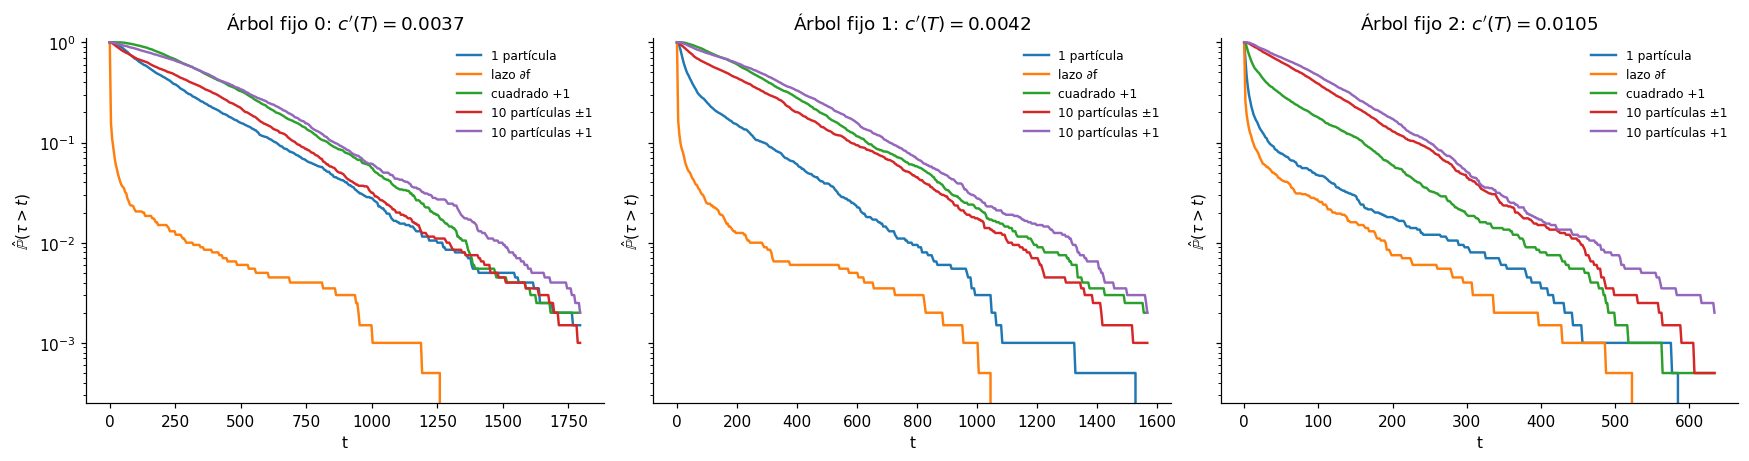
\includegraphics[width=\textwidth]{figuras/ext_arbol_fijo.png}
\caption{Supervivencia con árbol fijo, para tres árboles. En cada panel, las colas de todas las condiciones iniciales son paralelas.}
\label{fig:quenched}
\end{figure}

\subsection*{La tasa de extinción es la constante de Poincaré}

Se sortearon 40 árboles. Para cada uno estima $\gamma(T)$ más allá del cuantil 0.8, con 600 réplicas que parten del cuadrado $+1$, y calcula $c'(T)=\lambda_{\min}\big(\Delta^{\uparrow}|_{E\setminus T}\big)$. Resultados:
\begin{itemize}[nosep]
  \item $\gamma(T)$ varía en un factor $8.6$ entre árboles (de $0.0016$ a $0.0138$);
  \item $\log\gamma(T)$ y $\log c'(T)$ tienen correlación $0.95$, con pendiente $1.07$ (figura~\ref{fig:poincare}).
\end{itemize}
Empíricamente,
\[
\boxed{\;\gamma(T)\approx c'(T)=\lambda_{\min}\big(\Delta^{\uparrow}|_{E\setminus T}\big).\;}
\]
Es coherente con el drift $\Lgen I(\theta)=-\Delta^\uparrow_T\theta$: la media evoluciona como $\frac{d}{dt}\mathbb{E}\theta_t=-\Delta^\uparrow_T\,\mathbb{E}\theta_t$, cuyo modo más lento decae como $e^{-c't}$, y la extinción ocurre a esa misma tasa. \textbf{Es una conjetura natural para el paper}, porque refinaría el Teorema~2.4 y la Observación~3 identificando la tasa exacta de la cola. Notar que el Teorema~2.4 solo da una cota con constantes que dependen de $c'$; la simulación sugiere que la relación es una igualdad asintótica.

\begin{figure}[ht]
\centering
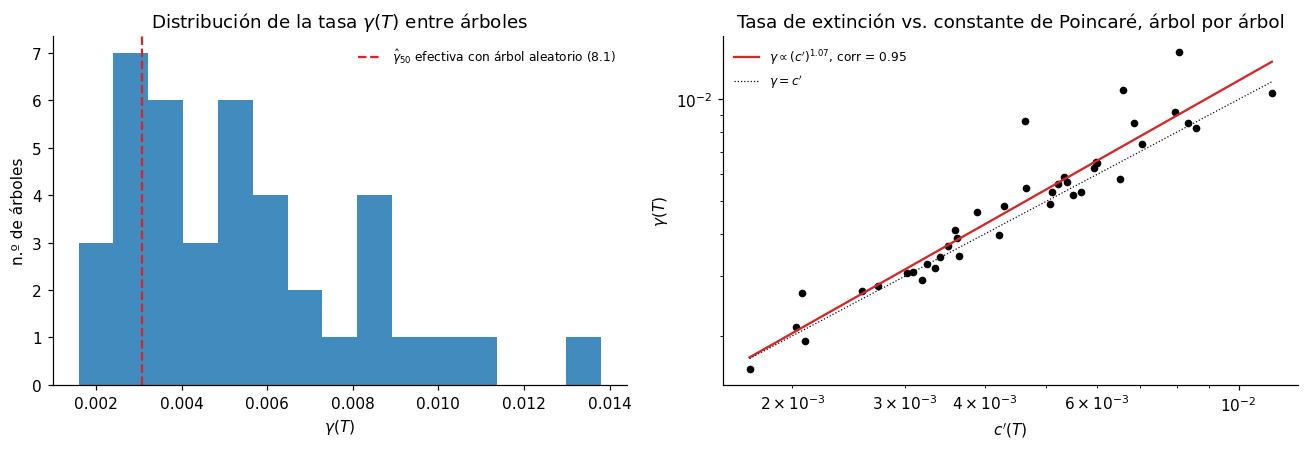
\includegraphics[width=\textwidth]{figuras/ext_gamma_poincare.png}
\caption{Izquierda: distribución de $\gamma(T)$ en 40 árboles; la línea roja es la tasa efectiva con árbol aleatorio. Derecha: $\gamma(T)$ frente a $c'(T)$ en escala log-log; la línea punteada es $\gamma=c'$.}
\label{fig:poincare}
\end{figure}

\section*{Referencias}
\begin{itemize}[nosep]
  \item D.~Cid, A.~Sepúlveda. \emph{Branching process on complexes}, borrador V1 (2026).
  \item S.~Mukherjee, J.~Steenbergen. \emph{Random walks on simplicial complexes and harmonics}. Random Structures \& Algorithms (2016).
  \item A.~M.~Duval, C.~J.~Klivans, J.~L.~Martin. \emph{Simplicial matrix-tree theorems}. Trans.\ AMS (2009).
  \item T.~M.~Liggett. \emph{Interacting Particle Systems}. Springer (1985).
  \item D.~T.~Gillespie. \emph{Exact stochastic simulation of coupled chemical reactions}. J.\ Phys.\ Chem.\ (1977).
  \item P.~Collet, S.~Martínez, J.~San Martín. \emph{Quasi-Stationary Distributions}. Springer (2013).
  \item E.~B.~Wilson. \emph{Probable inference, the law of succession, and statistical inference}. J.\ Amer.\ Statist.\ Assoc.\ (1927).
  \item L.~D.~Brown, T.~T.~Cai, A.~DasGupta. \emph{Interval estimation for a binomial proportion}. Statistical Science (2001).
  \item R.~E.~Tarjan. \emph{Efficiency of a good but not linear set union algorithm}. J.\ ACM (1975).
\end{itemize}

\end{document}
